% Options for packages loaded elsewhere
\PassOptionsToPackage{unicode}{hyperref}
\PassOptionsToPackage{hyphens}{url}
\PassOptionsToPackage{dvipsnames,svgnames,x11names}{xcolor}
%
\documentclass[
  letterpaper,
  DIV=11,
  numbers=noendperiod]{scrreprt}

\usepackage{amsmath,amssymb}
\usepackage{iftex}
\ifPDFTeX
  \usepackage[T1]{fontenc}
  \usepackage[utf8]{inputenc}
  \usepackage{textcomp} % provide euro and other symbols
\else % if luatex or xetex
  \usepackage{unicode-math}
  \defaultfontfeatures{Scale=MatchLowercase}
  \defaultfontfeatures[\rmfamily]{Ligatures=TeX,Scale=1}
\fi
\usepackage{lmodern}
\ifPDFTeX\else  
    % xetex/luatex font selection
\fi
% Use upquote if available, for straight quotes in verbatim environments
\IfFileExists{upquote.sty}{\usepackage{upquote}}{}
\IfFileExists{microtype.sty}{% use microtype if available
  \usepackage[]{microtype}
  \UseMicrotypeSet[protrusion]{basicmath} % disable protrusion for tt fonts
}{}
\makeatletter
\@ifundefined{KOMAClassName}{% if non-KOMA class
  \IfFileExists{parskip.sty}{%
    \usepackage{parskip}
  }{% else
    \setlength{\parindent}{0pt}
    \setlength{\parskip}{6pt plus 2pt minus 1pt}}
}{% if KOMA class
  \KOMAoptions{parskip=half}}
\makeatother
\usepackage{xcolor}
\ifLuaTeX
  \usepackage{luacolor}
  \usepackage[soul]{lua-ul}
\else
  \usepackage{soul}
  
\fi
\setlength{\emergencystretch}{3em} % prevent overfull lines
\setcounter{secnumdepth}{5}
% Make \paragraph and \subparagraph free-standing
\makeatletter
\ifx\paragraph\undefined\else
  \let\oldparagraph\paragraph
  \renewcommand{\paragraph}{
    \@ifstar
      \xxxParagraphStar
      \xxxParagraphNoStar
  }
  \newcommand{\xxxParagraphStar}[1]{\oldparagraph*{#1}\mbox{}}
  \newcommand{\xxxParagraphNoStar}[1]{\oldparagraph{#1}\mbox{}}
\fi
\ifx\subparagraph\undefined\else
  \let\oldsubparagraph\subparagraph
  \renewcommand{\subparagraph}{
    \@ifstar
      \xxxSubParagraphStar
      \xxxSubParagraphNoStar
  }
  \newcommand{\xxxSubParagraphStar}[1]{\oldsubparagraph*{#1}\mbox{}}
  \newcommand{\xxxSubParagraphNoStar}[1]{\oldsubparagraph{#1}\mbox{}}
\fi
\makeatother


\providecommand{\tightlist}{%
  \setlength{\itemsep}{0pt}\setlength{\parskip}{0pt}}\usepackage{longtable,booktabs,array}
\usepackage{calc} % for calculating minipage widths
% Correct order of tables after \paragraph or \subparagraph
\usepackage{etoolbox}
\makeatletter
\patchcmd\longtable{\par}{\if@noskipsec\mbox{}\fi\par}{}{}
\makeatother
% Allow footnotes in longtable head/foot
\IfFileExists{footnotehyper.sty}{\usepackage{footnotehyper}}{\usepackage{footnote}}
\makesavenoteenv{longtable}
\usepackage{graphicx}
\makeatletter
\newsavebox\pandoc@box
\newcommand*\pandocbounded[1]{% scales image to fit in text height/width
  \sbox\pandoc@box{#1}%
  \Gscale@div\@tempa{\textheight}{\dimexpr\ht\pandoc@box+\dp\pandoc@box\relax}%
  \Gscale@div\@tempb{\linewidth}{\wd\pandoc@box}%
  \ifdim\@tempb\p@<\@tempa\p@\let\@tempa\@tempb\fi% select the smaller of both
  \ifdim\@tempa\p@<\p@\scalebox{\@tempa}{\usebox\pandoc@box}%
  \else\usebox{\pandoc@box}%
  \fi%
}
% Set default figure placement to htbp
\def\fps@figure{htbp}
\makeatother

\usepackage[makeroom]{cancel}
\usepackage{makeidx}
\makeindex
\KOMAoption{captions}{tableheading}
\makeatletter
\@ifpackageloaded{bookmark}{}{\usepackage{bookmark}}
\makeatother
\makeatletter
\@ifpackageloaded{caption}{}{\usepackage{caption}}
\AtBeginDocument{%
\ifdefined\contentsname
  \renewcommand*\contentsname{Índice}
\else
  \newcommand\contentsname{Índice}
\fi
\ifdefined\listfigurename
  \renewcommand*\listfigurename{Lista de Figuras}
\else
  \newcommand\listfigurename{Lista de Figuras}
\fi
\ifdefined\listtablename
  \renewcommand*\listtablename{Lista de Tabelas}
\else
  \newcommand\listtablename{Lista de Tabelas}
\fi
\ifdefined\figurename
  \renewcommand*\figurename{Figura}
\else
  \newcommand\figurename{Figura}
\fi
\ifdefined\tablename
  \renewcommand*\tablename{Tabela}
\else
  \newcommand\tablename{Tabela}
\fi
}
\@ifpackageloaded{float}{}{\usepackage{float}}
\floatstyle{ruled}
\@ifundefined{c@chapter}{\newfloat{codelisting}{h}{lop}}{\newfloat{codelisting}{h}{lop}[chapter]}
\floatname{codelisting}{Listagem}
\newcommand*\listoflistings{\listof{codelisting}{Lista de Listagens}}
\makeatother
\makeatletter
\makeatother
\makeatletter
\@ifpackageloaded{caption}{}{\usepackage{caption}}
\@ifpackageloaded{subcaption}{}{\usepackage{subcaption}}
\makeatother

\ifLuaTeX
\usepackage[bidi=basic]{babel}
\else
\usepackage[bidi=default]{babel}
\fi
\babelprovide[main,import]{portuguese}
% get rid of language-specific shorthands (see #6817):
\let\LanguageShortHands\languageshorthands
\def\languageshorthands#1{}
\usepackage[]{biblatex}
\addbibresource{references.bib}
\usepackage{bookmark}

\IfFileExists{xurl.sty}{\usepackage{xurl}}{} % add URL line breaks if available
\urlstyle{same} % disable monospaced font for URLs
\hypersetup{
  pdftitle={Cálculo Companheiro},
  pdfauthor={Artur H. Tomita, Eduardo Yukio G. Ishihara, Gustavo S. Garone},
  pdflang={pt},
  colorlinks=true,
  linkcolor={blue},
  filecolor={Maroon},
  citecolor={Blue},
  urlcolor={Blue},
  pdfcreator={LaTeX via pandoc}}


\title{Cálculo Companheiro}
\author{Artur H. Tomita, Eduardo Yukio G. Ishihara, Gustavo S. Garone}
\date{2025-02-21}

\begin{document}
\maketitle

\renewcommand*\contentsname{Índice}
{
\hypersetup{linkcolor=}
\setcounter{tocdepth}{2}
\tableofcontents
}

\bookmarksetup{startatroot}

\chapter*{Calculo Companheiro}\label{calculo-companheiro}
\addcontentsline{toc}{chapter}{Calculo Companheiro}

\markboth{Calculo Companheiro}{Calculo Companheiro}

\newcommand{\pt}[3]{\frac{\partial^2{#1}}{\partial{#2}\partial{#3}}}
\newcommand{\ptd}[3]{\left. \frac{\partial^2{#1}}{\partial{#2}\partial{#3}} \right \rvert_{(x_0,y_0)}}

\section*{Propósito do Livro}\label{propuxf3sito-do-livro}
\addcontentsline{toc}{section}{Propósito do Livro}

\markright{Propósito do Livro}

Esse livro foi criado com inteção de fornecer um material acessível a
estudantes da graduação para seus estudos de Cálculo introdutório
(Cálculo I) e multivariado (Cáculo II).

Buscamos escrever esse livro com uma linguagem metematicamente mais
acessível, usando de paralelos, exemplos e construções a partir de
simplficiações para desenvolvermos a intuição matemática do leitor,
ponto chave no desempenho de qualquer pessoa nas matérias de exatas.
Temos como principal alvo alunos no primeiro ano da graduação nos cursos
de exatas, quando são expostos pela primeira vez ao Cálculo, ou aos
publicos de outros cursos que frequentam a matéria.

Esse livro é aberto para uso por toda a comunidade e possui pouco ou
nenhum material de uso restrito ou de código fechado, conforme as
recomendações da \textcite{unesco_recomendacao_2022} para a ciência
aberta.

\section*{Como usar esse livro}\label{como-usar-esse-livro}
\addcontentsline{toc}{section}{Como usar esse livro}

\markright{Como usar esse livro}

Como esse livro foi pensado para servir de referência e suporte das
matérias de cálculo, você pode não ver muita vantagem em ler o livro
``de cabo a rabo'', e sim em consultar o que você está com dificuldade
ou não conseguiu assimilar muito bem em aula. Uma boa forma de usar esse
livro é ler nosso capítulo sobre determinado assunto que você gostaria
de estudar e então partir para material mais ``pesado'', como os livros
de cálculo do Guidorizzi, Stewart, Apostol e afins.

Busque no sumário (ou, na versão online, a tabela de conteúdos à
esquerda) pelo conteúdo desejado. Caso queira algo mais específico, como
algum teorema específico ou conceito que não conseguiu encontrar pelos
títulos dos capítulos, consulte o índice no fim do livro.

\section*{Quem Somos}\label{quem-somos}
\addcontentsline{toc}{section}{Quem Somos}

\markright{Quem Somos}

Esse livro foi escrito pelos alunos do Bacharelado em Estatística do
IME-USP, Gustavo S. Garone e Eduardo Yukio G. Ishihara Sob supervisão do
\href{https://www.ime.usp.br/~tomita/}{Prof.~Artur Hideyuki Tomita} do
departamento de matemática do IME-USP.

Você pode nos contatar via email em
\href{mailto:gustavo.garone@usp.br}{gustavo.garone arroba usp.br}

\section*{Agradecimentos}\label{agradecimentos}
\addcontentsline{toc}{section}{Agradecimentos}

\markright{Agradecimentos}

Esse projeto foi parcialmente financiado pelo
\href{https://prip.usp.br/pub/}{Programa Unificado de Bolsas} da
Universidade de São Paulo.

\bookmarksetup{startatroot}

\chapter*{Prefácio}\label{prefuxe1cio}
\addcontentsline{toc}{chapter}{Prefácio}

\markboth{Prefácio}{Prefácio}

Resumo dos conteudos do livro, ou seja, um sumário.

\part{Bem-Vindo!}

\chapter{Introdução}\label{introduuxe7uxe3o}

\section{Apresentação do material}\label{apresentauxe7uxe3o-do-material}

Bom dia, boa tarde, boa noite e, para os desesperados, boa madrugada! 👋

Este material de apoio aos estudo e preparação para as disciplinas de
Cálculo I e II foi financiado pelo
\href{https://prip.usp.br/pub/}{Programa Unificado de Bolsas} como um
projeto de ensino do \href{https://www.ime.usp.br/~tomita/}{Professor
Dr.~Artur Hideyuki Tomita} e produzido pelos discentes
\href{gustavo.garone@usp.br}{Gustavo Silva Garone} e
\href{eduardoyukio.ishihara@usp.br}{Eduardo Yukio G. Ishihara}, ambos do
Instituto de Matemática e Estatística (🔴⚪). Por favor, sinta-se livre
para enviar-nos um e-mail com correções, recomendações, elogios ou
críticas. Este projeto está constantemente sendo produzido, mantido e
corrigido, então ficaremos mais do que felizes em receber sua opinião.

Independentemente se este é o seu primeiro ano ou não da faculdade,
muito provavelmente já ouviu atrocidades sobre \st{o terror dos cursos
de exatas} Cálculo Diferencial e Integral. É exatamente por conta dessa
mística construída ao redor de uma das disciplinas mais fundamentais
para a matemática que nasce o projeto. Somos estudantes fazendo um
material para estudantes (sob a supervisão de um professor), o que nos
dá uma visão muito mais próxima da real experiência que você, leitor,
provavelmente está passando agora. Buscamos o equilíbrio entre o rigor
exigido pelo fazer matemático e a informalidade que gera interesse.

Para todos os tópicos, tentaremos apresentá-los seguindo uma sequência
lógica e didática composta por uma introdução fundamentada na sua
intuição, algumas aplicações reais do tópico para os diversos cursos,
introdução à teoria, formalização da teoria, formalização dos exemplos,
alguns exercícios de apoio e, por fim, soluções comentadas. Uma segunda
característica notável no material é a divisão dos temas em
``importantes'' e ``opcionais''. Por mais que sejamos obrigados a dizer
que todos os tópicos da matéria são igualmente importantes em sua
íntegra, alguns terão menor aplicações e outros serão frequentemente
requeridos em matérias futuras.

Finalmente, sempre que possível, apresentaremos interpretações
alternativas aos conceitos debatidos em cada tópico. Por exemplo, no
estudo do determinante de matrizes, trataremos os determinantes primeiro
como uma construção algébrica, pois, apesar de abstrato, é mais direto e
é o mínimo necessário para a sua aplicação, apesar de raso, e, em
seguida, apresentaremos o determinante sob uma perspectiva geométrica,
que é um primeiro contato com a algebra linear e as transformações
lineares.

\section{Estudando Matemática}\label{estudando-matemuxe1tica}

Se você é do IME, este tópico provavelmente estendê-se-á a quase todas
as outras matérias, mas, para os outros institutos, o estudo rigoros da
matemática pode ser um tópico exótico até agora. Uma parte significativa
dos docentes diria que as notas devem ser a menor preocupação do aluno e
que o verdadeiro objetivo da disciplina é aprender o conteúdo e, se
possível, divertir-se no processo, mas sabemos que tal realidade é muito
distante para quase todos nós meros mortais.

\subsection{A aquisição da
Intuição}\label{a-aquisiuxe7uxe3o-da-intuiuxe7uxe3o}

Aprender matemática ocorre por meio do entendimento dos processos e pelo
desenvolvimento disto que podemos chamar de ``intuição matemática''.
Considere o seguinte problema:

\begin{quote}
Um laboratório de química contém tubos de ensaios idênticos e não
identificados. Cada tubo de ensaio contém 5g ou 8g de um sal. Um
estudante chegou ao laboratório e notou que 10 tubos estavam vazios e o
seus conteúdos foram depositado em um becker. Após os devidos
procedimentos, o estudante constatou que havia 59g do sal no becker.
Quantos tubos de cada tipo foram usados?
\end{quote}

Apesar de nunca ter visto este exato problema antes, não é difícil
perceber que ele requer um sistema linear não homogêneo (tudo bem se
você não compreende muito bem o que todas essas palavras querem dizer) e
conclua que foram usados 7 tubos de 5g e 3 tubos de 8g. O seu primeiro
passo para resolver o problema foi, muito provavelmente, lê-lo. Em
seguida, sua intuição e sua experiência indicaram que a estrutura do
problema assemelha-se aos problemas de sistemas lineares vistos
anteriormente na sua vida. Então, você aplicou os valores corretos e
atribuiu as variáveis corretas para montar e sistema e, por fim,
resolveu-o utilizando o seu método favorito. Tudo isso ocorre sem que
você tenha, necessariamente, notado. Essa é a ``intuição matemática''.

Alternativamente, algumas pessoas podem ter resolvido com um método
alternativo de Cálculo Hipotético Universal Técnico Estimativo (CHUTE),
mas saiba que também há muita intuição por trás disso! Teoricamente,
havia infinitas possibilidades para serem ``chutadas''. Como sabemos que
\(\pi\) não é a resposta? E, talvez, \((5.2, 8, 5, \sqrt{5}, 3)\)?
Chutar 7 tubos de 5g e 3 tubos de 8g não é tão óbvio (evitaremos essa
palavra no decorrer do texto por motivos óbvios) quanto pode parecer,
apesar do problema ser simples. Para chegar à resposta, a pessoa deve
compreender algumas coisas:

\begin{itemize}
\tightlist
\item
  A resposta deve ser o número de tubos de 8g e o número de tubos de 5g
  (dois números ao todo)
\item
  O número de tubos é um número natural (inteiro não negativo)
\item
  8 vezes o número de tubos de 8g mais 5 vezes o número de tubos de 5g é
  igual a 65g
\end{itemize}

Acredite ou não, você também chegou a todas essas conclusões sem nem
pensar sobre! Parabéns, esse é o passo fundamental para a nossa jornada
de aprender matemática, em especial Cálculo I e II!

\subsection{A prática leva à
perfeição}\label{a-pruxe1tica-leva-uxe0-perfeiuxe7uxe3o}

A próxima lição sobre o aprendizado da matemática pode soar repetitiva,
mas gostaríamos de lembrar: apender matemática é um processo muito
difícil de ser acelerado. Tentar aprender um conteúdo na noite antes da
prova é como tentar pegar uma faca caindo: pode ser um feito sensacional
ou uma épica tragédia! Apesar de defendermos o papel da intuição no
fazer matemáico, não podemos estar limitados a ela e é daí que surge o
rigor matemático. Quando formalizamos um conceito, ganhamos a capacidade
de facilmente aplicar aquele método em situações semelhantes e
conseguimos explorar até o extremo. É assim que muitas das áreas da
matemática foram criadas (ou descobertas). Primeiro, você aprendeu a
``tirar a raiz quadrada'' de números quadrados perfeitos (1, 4, 9,
25\ldots). Depois, estendeu o conceitos para outros números inteiros o
que gerou o conjunto dos números irracionais (aqueles que não podem ser
escritos como uma fração de inteiros). Por fim, pode ter estendido a
raiz quadrada para os números negativos, o que gerou o conjuntos dos
números imaginários (fique tranquilo, pois este não é um conteúdo
obrigatório para cálculo, mas ainda assim preparamos uma sessão dedicada
a eles).

Uma boa prática é dedicar uma hora de estudo para essa disciplina nos
dias em que ela é oferecida, assim como para as outras matérias. Se
possível, revise a matéria, faça exercícios indicados pelo professor ou
os que escontrar neste material, estude em grupo e, acima de tudo, ajude
seus colegas. Ensinar outra pessoa é uma das melhores maneiras de fixar
e testa os seus conhecimentos, além de ajudar uma pessoa que
provavelmente não entendeu o conteúdo tão rapidamente quanto você!

\section{Hora de começarmos!}\label{hora-de-comeuxe7armos}

A você, que dedicou seu tempo a ler as dicas e os textos introdutórios,
devemos agradecer, é você em quem investimos \st{muitas} horas na
produção do material e esperamos que a sua experiência com cálculo deixe
de ser a história de terror contada por muitos veteranos e torne-se uma
agradável introdução ao fazer matemático!

Nos vemos nos próximos capítulos! 🤩

\part{Matemática Elementar}

\chapter{Funções Polinomiais}\label{funuxe7uxf5es-polinomiais}

\section{Introdução}\label{introduuxe7uxe3o-1}

Neste, capítulo, daremos início ao estudo de funções polinomiais, ou
apenas polinômios daqui para frente. Funções polinomiais são um conjunto
de funções muito bem definidas e simples, o que torna-as adequadas para
modelar situações extremamente variadas. Ademais, funções polinomiais
geralmente são as funções mais simples que podemos trabalhar em diversos
contextos (desde cálculo a modelagem de dados), então serão as primeiras
funções a efetivamente aprofundarmos!

Vamos ver alguns exemplos:

\begin{quote}
1- Um projétil foi atirado de um canhão de cima de uma plataforma. Um
físico determinou que a altura do objeto, em função do tempo após o
lançamento, pode ser descrita por \(h(t) = 4.9t^2+100t+8\)
\end{quote}

\begin{quote}
2- Após analisar o valor das ações de uma empresa, um economista
determinou que a \href{https://pt.wikipedia.org/wiki/Média_móvel}{média
móvel} dos valores do ativo, em função do tempo, pode ser modelado por
\(v(t) = −0.0002t^3+31.664t^2–10^6t+2×1010\)
\end{quote}

\begin{quote}
3- Uma bióloga, ao medir várias vezes o volume de oxigênio (em unidade
desconhecida) produzido por uma população de algas, notou que a produção
variava de acordo com a concentração de algas em seu aquário. A
concentração variava de 0 gramas de algas por L a 100g de algas por
litro. A biólogo notou que a produção era modelada pela função
\(p(c) = \frac{-5}{1000}(c^2-120c)\)
\end{quote}

\begin{quote}
4- Um triatleta precisa atravessar de um lado de um lago para o outro.
Sua velocidade em terra é diferente da velocidade em água e a distância
em terra é de 50m. Seu preparador físico modelou o problema e determinou
que o tempo gasto para chegar ao destino, em função da distância
percorrida em terra é dado pelo polinômio
\(t(d) = \frac{d^2}{20}-\frac{11d}{4}+85\)
\end{quote}

Estes dois últimos exemplos utilizam um polinômio para modelar uma
situação, mas é fácil perceber que o grande objetivo por trás dos
experimentos é maximizar a produção de oxigênio e minimizar o tempo
gasto. Tal classe de problemas recebe o nome de \textbf{Problemas de
Otimização} e será tratado num capítulo a parte, pois o estudo rigoroso
requer o uso de derivadas. Por agora, ao tentarmos encontrar estes
pontos de máximo e mínimo, vamos recorrer a um método mais rudimentar:
olhar o gráfico.

Até agora, tivemos um contato inicial com os polinômios e apenas uma
intuição do que eles são. Analisando os polinômios obtidos em cada
exemplo, você deve ter notado algumas características comuns. Portanto,
vamos dar início à formalização dessa intuição!

\section{Anatomia de um polinômio de uma
variável}\label{anatomia-de-um-polinuxf4mio-de-uma-variuxe1vel}

Primeiro, vamos definir a parte mais fundamental de uma função: seu
domínio e contradomínio. Polinômios são funções cujo domínio são os
complexos e o contradomínio também são os complexos:
\(f(x): \mathbb{C} \to\mathbb{C}\) (lê-se ``f de x leva de complexos em
complexos'').

A palavra ``polinômio'' vem da junção de ``\emph{poli}'', que vem do
grego e significa ``muitos'' e ``\emph{nomen}'', que vem do latim e
significa ``nome'', ou, mais vulgarmente, ``temo''. Em suma, polinômios
são várias coisas! Vamos, agora, à definição de fato.

\begin{quote}
Polinômios são expressões que podem ser construídas a partir de
constantes e variáveis por meio de soma, subtração, multiplicação e
exponenciação por inteiros não negativos.
\end{quote}

Ou seja, de forma genérica, um polinômio de x é da forma \[
p(x) = a_{n}x^{n} + a_{n-1} x^{n-1} + \dots + a_{2}x^{2}+a_{1}x+a_{0} = \sum_{i=0}^{n} a_{i} x^{i}
\]

Apesar de não explicitados, perceba que \(a_1x = a_1x^1\) e
\(a_0 = a_0x^0 = a_0\times1\).

Note que todos os termos \(a_i\) são números e os expoentes também são
números. É importante garantir tal fato, pois pode gerar problemas ao
definirmos o grau do polinômio e ao verificarmos outras propriedades, um
\(x\) no expoente gera uma função exponencial, não uma polinomial!

Todavia, como nem tudo na matemática são flores, polinômios nem sempre
terão a cara de polinômios. Veja os exemplos abaixo:

\begin{quote}
\(f(x) =\frac{x^2-1}{x+1}\), com \(x\neq1\)

\(f(x)=\frac{x^2-1}{x+1}=  \frac{(x+1)(x-1)}{(x+1)} =x-1\)

Portanto, \(f(x) = \frac{x^2-1}{x+1}\), com \(x\neq1\) é um polinômio.
\end{quote}

\begin{quote}
\(f(x)=tg(arctg(5x^2-\pi))\)

\(f(x) = tg(arctg(5x^2-\pi))) = 5x^2-\pi\)

Portanto, \(f(x)=tg(arctg(5x^2-\pi))\) é um polinômio.
\end{quote}

No exemplo acima, tome muito cuidado ao manipular funções
trigonométricas. \(tg(arctg(f(x))=f(x)\), mas \(arctg(tg(f(x))\) nem
sempre é igual a \(f(x)\). Isso ocorre por conta dos domínios das
funções e onde podem ser invertidas, mas tal assunto é tratado em outro
capítulo.

\begin{quote}
\(f(x) = e^{ln(5 x^{-1})}\)

\(f(x) = e^{ln(5 x^{-1})} = 5x^{-1}\)

Portanto, \(f(x) = e^{ln(5 x^{-1})}\) não é um polinômio, pois o \(x\)
tem um expoente negativo, ou seja, não é positivo nem nulo.
\end{quote}

Determinar se uma função é polinomial trata-se, portanto, de verificar
se aquela função pode ser reescrita como uma soma de potências de \(x\)
multiplicadas por uma constante. Neste momento, trataremos apenas de
polinômios com quantidade finita de termos. O uso de polinômios com
infinitos termos, apesar de parecer pouco intuitivo, é uma técnica muito
usada para aproximar funções genéricas por um polinômio, o que tem
aplicações nas mais diversas áreas, sobretudo na computação.

\subsection{Grau de um polinômio}\label{grau-de-um-polinuxf4mio}

O grau de um polinômio, notado \(gr(P)\) ou \(grau(P)\), refere-se ao
maior expoente da variável. Genericamente, temos que o grau de um
polinômio é \(n\) tal que \(a_n \neq 0\). Ou seja, o maior número ao
qual \(x\) está sendo elevado, quando trata-se de um polinômio em \(x\)
e a constante não é 0.

Particularmente, alguns polinômios de grau pequeno recebem alguns nomes
especiais.

\begin{longtable}[]{@{}rl@{}}
\toprule\noalign{}
Grau do Polinômio & Nome do Polinômio \\
\midrule\noalign{}
\endhead
\bottomrule\noalign{}
\endlastfoot
0 & Constante \\
1 & Linear \\
2 & Quadrático \\
3 & Cúbico \\
\end{longtable}

Um polinômio constante é, simplesmente, um número, ou seja, \(p(x)=a_0\)
e seu gráfico é uma linha horizontal que intercepta o eixo \(y\) no
ponto \((0,a_0)\).

Um polinômio linear é da forma \(p(x) = a_1x+a_0\). Ele intercepta o
eixo \(y\) no ponto \((0,a_0)\). Seu gráfico é uma reta não paralela a
nenhum dos eixos.

Um polinômio quadrático é da forma \(p(x) = a_2x^2+a_1x+a_0\). Você já
deve imaginar onde ele intercepta o eixo \(y\). O gráfico de um
polinômio quadrático é uma parábola.

Um polinômio cúbico é da forma \(p(x) = a_3x^3+a_2x^2+a_1x+a_0\). Mais
uma vez, não é difícil inferir onde ele intercepta o eixo \(y\). Seu
gráfico pode variar de acordo com os parâmetros, mas geralmente forma
uma letra ``n'' e explode para infinito positivo e infinito negativo em
cada uma das suas extremidades.

Polinômios de grau superior não recebem nomes especiais, pois são menos
frequentemente trabalhados em aula e não têm propriedades facilmente
generalizadas, como é o caso da parábola e a reta.

\subsection{Raízes de um Polinômio}\label{rauxedzes-de-um-polinuxf4mio}

Encontrar as raízes de um polinômio nada mais é do que encontrar os
pontos em que \(p(x) = 0\), ou seja, quando o polinômio intercepta o
eixo \(x\).

Encontrar as raízes de um polinômio é um processo cujo trabalho cresce
exponencialmente de acordo com o grau do polinômio, por isso traremos
algumas técnicas algorítmicas para encontrar as raízes, fórmulas e
intuições. No futuro, com o Teorema do Valor Intermediário, o processo
de encontrar as raízes de um polinômio pode tornar-se mais fácil (e
bonito), mas nunca trivial!

\subsubsection{Para polinômios de grau
0:}\label{para-polinuxf4mios-de-grau-0}

Um polinômio de grau 0 pode ter zero raízes ou infinitas raízes! Quando
\(a_0=0\), o polinômio coincide com o eixo \(x\) em todos os pontos,
portanto todos os pontos são raízes e há infinitos sobre sobre o eixo
\(x\). Quando \(a_0 \neq 0\), o polinômio é paralelo ao eixo\(x\) e não
coincidente, portanto \(p(x)\) nunca é igual a \(0\), ou seja, não há
nenhuma raiz.

\subsubsection{Para polinômios de grau
1:}\label{para-polinuxf4mios-de-grau-1}

\(p(x) = a_1x+a_0 =0 \Leftrightarrow a_1x=-a_0 \Leftrightarrow x = -\frac{a_0}{a_1}\)
A única raiz de um polinômio de grau 1 é \(x=-\frac{a_0}{a_1}\)

\subsubsection{Para polinômios de grau
2:}\label{para-polinuxf4mios-de-grau-2}

Para achar as raízes de um polinômio de grau 2, temos uma fórmula muito
conhecida por nós brasileiros: a fórmula de Bhaskara, que não foi
descoberta por
\href{https://pt.wikipedia.org/wiki/F\%C3\%B3rmula_quadr\%C3\%A1tica\#Desenvolvimento_hist\%C3\%B3rico}{Bhaskara}.
Segue aqui uma demonstração da fórmula: \[
\begin{aligned}
    p(x) &= a_2x^2+a_1x+a_0 = 0 \\
    &\Leftrightarrow \dfrac{a_2x^2+a_1x+a_0}{a_2} = \dfrac{0}{a^2} \\
    &\Leftrightarrow x^2 + \dfrac{a_1x}{a_2} + \dfrac{a_0}{a_2} = 0 \\
    &\Leftrightarrow x^2 + \dfrac{a_1x}{a_2} = - \dfrac{a_0}{a_2} \\
    &\Leftrightarrow x^2 + \dfrac{a_1x}{a_2} + \left(\dfrac{a_1}{2a_2}\right)^2 = - \dfrac{a_0}{a_2}+\left(\dfrac{a_1}{2a_2}\right)^2 \\
    &\Leftrightarrow x^2 + \dfrac{a_1x}{a_2} + \dfrac{{a_1}^2}{4{a_2}^2} = - \dfrac{a_0}{a_2}+\dfrac{{a_1}^2}{{4a_2}^2}
\end{aligned}
\]

Trata-se de um produto notável! \[
\begin{aligned}
    &\Leftrightarrow  \left(x+\dfrac{a_1}{2a_2}\right)^2 = - \dfrac{a_0}{a_2}+\dfrac{{a_1}^2}{{4a_2}^2} \\
    &\Leftrightarrow  \left(x+\dfrac{a_1}{2a_2}\right)^2 = \dfrac{{a_1}^2-4 \cdot a_0 \cdot a_2}{{4a_2}^2} \\
    &\Leftrightarrow  \sqrt{\left(x+\dfrac{a_1}{2a_2}\right)^2}=\sqrt{ \dfrac{{a_1}^2-4 \cdot a_0 \cdot a_2}{{4a_2}^2}} \\
    &\Leftrightarrow  x+\dfrac{a_1}{2a_2} = \pm \sqrt{ \dfrac{{a_1}^2-4 \cdot a_0 \cdot a_2}{{4a_2}^2}} \\
    &\Leftrightarrow  x+\dfrac{a_1}{2a_2} = \pm { \dfrac{\sqrt{{a_1}^2-4 \cdot a_0 \cdot a_2}}{\sqrt{{4a_2}^2}}} \\
    &\Leftrightarrow  x+\dfrac{a_1}{2a_2} = \pm { \dfrac{\sqrt{{a_1}^2-4 \cdot a_0 \cdot a_2}}{2a_2}} \\
    &\Leftrightarrow  x = \pm { \dfrac{\sqrt{{a_1}^2-4 \cdot a_0 \cdot a_2}}{2a_2}}-\dfrac{a_1}{2a_2} \\
    &\Leftrightarrow  x = { \dfrac{-a_1 \pm\sqrt{{a_1}^2-4 \cdot a_0 \cdot a_2}}{2a_2}}
\end{aligned}
\]

\(p(x) = a_2x^2+a_1x+a_0 = ax^2+bx+c\)

Renomeamos as variáveis acima apenas para facilitar a sua identificação
dos termos em relação ao padrão usado no ensino médio. Portanto,
\(x = \dfrac{-b \pm \sqrt{b^2-4 \cdot a \cdot c }}{2a}\)

Tomando \(\Delta = b^2-4 \cdot a \cdot c\) :
\(x=\dfrac{-b \pm \sqrt{\Delta}}{2a}\)

Da fórmula, segue que, quando \(\Delta>0\), o polinômio tem duas raízes
reais, quando \(\Delta=0\), o polinômio só tem uma raiz distinta, quando
\(\Delta<0\), o polinômio não tem nenhuma raiz real.

Por agora, preste muita atenção quando dizemos ``o polinômio só tem uma
raiz distinta'' e ``o polinômio não tem nenhuma raiz real'', pois em
breve tais fatos não nos impedirão de fazer mais contas!

\subsection{Para polinômios de grau maior que
2:}\label{para-polinuxf4mios-de-grau-maior-que-2}

Existe \href{https://en.wikipedia.org/wiki/Galois_theory}{um ramo da
matemática} que nasceu do estudo das raízes de um polinômio. Desta área,
trazemos a você, leitor, um resultado muito triste: não existe uma
fórmula para as raízes de um polinômio de grau 5 ou superior. Todavia,
para grau 3 e 4 há fórmulas explicitadas a partir dos coeficientes do
polinômio. Para a alegria de todos, tais fórmulas são muito grandes para
trazermos nesse material ou para você encontrar uma aplicação para elas.

\begin{quote}
Mas o que fazer se eu precisar achar as raízes de um polinômio de grau 3
ou maior?
\end{quote}

Não se preocupe, a próxima seção dedicar-se-á exclusivamente a métodos
alternativos para achar a raiz sem o uso de fórmulas como as anteriores.

\chapter{Matrizes}\label{matrizes}

Uma matriz \(m \times n\) (lemos: ``m por n'') tem \(m\) linhas, na
horizontal, e \(n\) colunas, na vertical. Também é comum usarmos
\(i \times j\), para indicar o tamanho ou \textbf{Ordem} da matriz.

Para indicar os elementos de uma matriz \(M_{m\times n}\), usamos a
mesma letra que indicamos a matriz, mas em caixa baixa. Ou seja, na
matriz \(M\) indicada abaixo, o elemento \(m_{2,3}\) é o elemento dessa
matriz que está na 2ª linha e 3ª coluna. Para indicar uma coluna ou
linha genérica, utilizamos o termo ``fileira''. \[
M_{m\times n}=
\begin{bmatrix}
    m_{1,1} & m_{1,2} & \dots & m_{1,n} \\
    m_{2,1} & m_{2,2} & \dots & m_{2,n} \\
    \vdots  & \vdots & \ddots & \vdots \\
    m_{m,1} & m_{m,2} & \dots & m_{m_n}
\end{bmatrix}
\]

\section{Igualdade de Matrizes}\label{igualdade-de-matrizes}

Duas matrizes são ditas iguais se, e somente se, elas têm os mesmo
tamanho e todos os elementos correspondentes são iguais. \[
A_{m\times n} = B_{o\times p} \Leftrightarrow
\begin{cases}
    a_{1,1} = b_{1,1} \\
    a_{2,1} = b_{2,1} \\
    \vdots  \\
    a_{m,n} = b_{m,n}\\
    m = o \\
    n = p
\end{cases}
\]

Alternatimente, é possível expressar a afirmação acima com uma notação
matemática mais formal. Nos capítulos iniciais deste livro, oferecemos
mais de uma notação para acostumar o leitor à escrita matemática, mas,
em capítulos futuros, exibiremos exclusivamente a notação formal. Veja o
exemplo: \[
A_{m,n} = B_{o,p} \Leftrightarrow m=o \text{ e }  n=p \text{ e para todo }  i \in [1,m], j \in [1,n],  a_{i,j} = b_{i,j}
\]

Lê-se: ``A matriz \(A\), \(m\) por \(n\), é igual à matriz \(B\), \(o\)
por \(p\), se, e somente se, \(m\) é igual a \(o\) e \(n\) é igual a
\(p\) e, para todo elemento \(i\) pertencente ao conjuntno de 1 a \(m\)
e todo \(j\) pertencente ao conjunto de 1 a \(n\), o elemento \(a\)
\(i,j\) é igual ao elemento \(b\) \(i,j\).

\section{Matriz Quadrada}\label{matriz-quadrada}

Uma matriz é dita quadrada se, e somento se, o número de linhas é igual
ao número de colunas. \(A_{m,n}\) é quadrada \(\Leftrightarrow m=n\)

Nas matrizes quadradas, há elementos que chamamos de diagonal principal
e diagonal secundária. A diagonal principal é aquela que corre de
\(1,1\) até \(m,n\), enquanto a secundária é aquela que corre de \(1,n\)
até \(m,1\)

\section{Matriz Nula}\label{matriz-nula}

Uma matriz é dita nula se, e somente se, todos os seus elementos são
iguais a zero. Alternativamente, A é nula
\(\Leftrightarrow \forall a \in A, \; a = 0\) (lê-se: ``A é nula se, e
somente se, para todo elemento \(a\) pertencente à matriz \(A\), tal
elemento é igual a \(0\).''). Como notação de uma matriz nula,
utilizamos o próprio algarismo 0, mas com o índice correspondente ao
tamanho da matriz. \[
0_{3\times 2}=
\underbrace{\begin{bmatrix}
    0 & 0  \\
    0 & 0  \\
    0 & 0
\end{bmatrix}}_{2}\Bigg\} ~_{3}
\]

Por mais que seja possível diferenciar a matriz nula do número \(0\) por
conta do índice, recomendamos que sempre atentem-se a que tipo de objeto
matemática estamos trabalhando. Posteriormente, quando trabalharmos com
vetores e espaços vetoriais, encontraremos mais um objeto cuja notação é
\(0\). Sempre que possível, reforçaremos ou explicitaremos qual objeto
estamos lidando, mas tal diferenciação não estará presente na maioria
dos materiais que encontrará durante sua jornada acadêmica.

\section{Matriz Identidade}\label{matriz-identidade}

Uma matriz identidade é uma matriz quadrada com \(1\)'s em sua diagonal
e \(0\)'s como outros elementos. É comum chamarmos a matriz identidade
de ordem \(n\), ou seja, com \(n\) linhas e \(n\) colunas, de \(I_n\):
\[
I_{1} = 
\begin{bmatrix}
1
\end{bmatrix}
\]

\[
I_{n} =
\begin{bmatrix}
    1 & 0 & \dots & 0 \\
    0 & 1 & \dots & 0 \\
    \vdots  & \vdots & \ddots & \vdots \\
    0 & 0 & \dots & 1_{(a_{n,n})}
\end{bmatrix}
\]

Esse nome, ``identidade'', fará mais sentido quando discutirmos
multiplicação de matrizes.

\section{Soma e Subtração de
Matrizes}\label{soma-e-subtrauxe7uxe3o-de-matrizes}

Para somar ou subtrair matrizes, basta realizar a operação elemento por
elemento, obtendo uma nova matriz: \[
\begin{aligned}
    A_{i\times j}+B_{i\times j}&=
    \begin{bmatrix}
        a_{1,1} & a_{1,2} & \dots & a_{1,j} \\
        a_{2,1} & a_{2,2} & \dots & a_{2,j} \\
        \vdots  & \vdots & \ddots & \vdots \\
        a_{i,1} & a_{i,2} & \dots & a_{i,j}
    \end{bmatrix}
    +
    \begin{bmatrix}
        b_{1,1} & b_{1,2} & \dots & b_{1,j} \\
        b_{2,1} & b_{2,2} & \dots & b_{2,j} \\
        \vdots  & \vdots & \ddots & \vdots \\
        b_{i,1} & b_{i,2} & \dots & b_{i,j}
    \end{bmatrix}\\ \\
    &=
    \begin{bmatrix}
        a_{1,1} + b_{1,1} & a_{1,2} + b_{1,2} & \dots & a_{1,j} + b_{1,j} \\
        a_{2,1} + b_{2,1} & a_{2,2} + b_{2,2} & \dots & a_{2,j} + b_{2,j} \\
        \vdots  & \vdots & \ddots & \vdots \\
        a_{i,1} + b_{i,1} & a_{i,2} + b_{i,2} & \dots & a_{i,j} + b_{i,j}
    \end{bmatrix}
\end{aligned}
\]

Dessa forma, podemos nos perguntar o que aconteceria se tentássemos
somar uma matriz \(3\times 3\) por uma \(2 \times 2\). Pode parecer
intuitivo pensar que essa soma poderia ser feita, deixando a linha 3 e
coluna 3 da primeira matriz intacta, mas esse pensamento está incorreto.
\textbf{Aviso}: \emph{Podemos apenas somar e subtraír matrizes de mesma
ordem.}

\section{Multiplicação de matrizes por
escalar}\label{multiplicauxe7uxe3o-de-matrizes-por-escalar}

Chamamos de escalar um número (normalmente real, comumente chamado de
\(\lambda\)) que multiplica um vetor ou matriz. Para multiplicar uma
matriz por um escalar, multiplicamos todos seus elementos por ele, um a
um, idependentemente da sua ordem. Isso recebe o nome de produto por
escalar. \[
\lambda~ M_{m\times n}=
\lambda~
\begin{bmatrix}
    a_{1,1} & a_{1,2} & \dots & a_{1,n} \\
    a_{2,1} & a_{2,2} & \dots & a_{2,n} \\
    \vdots  & \vdots & \ddots & \vdots \\
    a_{m,1} & a_{m,2} & \dots & a_{m,n}
\end{bmatrix}
=
\begin{bmatrix}
    \lambda a_{1,1} & \lambda a_{1,2} & \dots & \lambda a_{1,n} \\
    \lambda a_{2,1} & \lambda a_{2,2} & \dots & \lambda a_{2,n} \\
    \vdots  & \vdots & \ddots & \vdots \\
    \lambda a_{m,1} & \lambda a_{m,2} & \dots & \lambda a_{m,n}
\end{bmatrix}
\]

\emph{Atenção}: Você pode já ter ouvido sobre \textbf{Produto Escalar}.
Isso \textbf{não} é o produto de uma matriz por um escalar, mas sim uma
operação distinta que estudaremos em algebra linear.

\emph{Produto Escalar}: Operação entre duas matrizes (vetores) que nos
dá um escalar \emph{Produto POR Escalar}: Operação que acabamos de
estudar entre matriz e um escalar que nos dá uma matriz. Conforme dito
anteriormente, compreender que tipo de objetos matemáticos estamos
trabalhando e quais operações podemos efetuar com eles é fundamental
para o estúdo do cálculo.

\section{Multiplicação de
Matrizes}\label{multiplicauxe7uxe3o-de-matrizes}

Para multiplicarmos duas matrizes, é necessário que o número de colunas
da primeira matriz seja igual ao número de linhas da segunda matriz. Por
esse e outros motivos, dizemos que a multiplicação de matrizes \emph{não
é comutativa}, ou seja, multiplicar uma matriz \(M\) por uma matriz
\(N\) pode nos dar uma matriz resultante diferente do que se
multiplicarmos \(N\) por \(M\), caso essa multiplicação seja se quer
possível! \[
\begin{aligned}
    M_{i\times j} \times N_{j\times k}, j=j \Rightarrow \checkmark \\
    M_{i\times j} \times B_{k\times j}, j\neq k \Rightarrow ✘ \\
    N_{j\times k} \times M_{i\times j}. k\neq i \Rightarrow ✘
\end{aligned}
\]

Vamos analisar como a operação é feita, e então nos ficará claro o
porquê dessa regra existir.

Considere as seguintes matrizes: \[
\begin{aligned}
    &A_{2\times 3} =
    \begin{bmatrix}
        1 & 2 & 3 \\
        4 & 5 & 6
    \end{bmatrix} \\ \\
    &B_{3\times 1} = 
    \begin{bmatrix}
        7 \\
        8 \\
        9
    \end{bmatrix}
\end{aligned}
\]

Sabemos que podemos multiplicá-las com A como primeira matriz
\(A_{2\times 3}\times B_{3\times 1}, 3=3\Rightarrow \checkmark\), mas
não como segunda matriz:
\(B_{3\times 1} \times A_{2\times 3}, 1\neq 2 \Rightarrow ✘\). Iremos
então realizar a primeira operação descrita da seguinte maneira:

\emph{Definição.} Para multiplicar matrizes, somaremos cada linha da
primeira multiplicada por um elemento equivalente de cada coluna: \[
\begin{aligned}
    &A \times B \\
    &=
    \begin{bmatrix}
        1 & 2 & 3 \\
        4 & 5 & 6
    \end{bmatrix}
    \times 
    \begin{bmatrix}
        7 \\
        8 \\
        9
    \end{bmatrix}\\ \\
    &=
    \begin{bmatrix}
        1 \cdot 7 + 2 \cdot 8 + 3 \cdot 9 \\
        4 \cdot 7 + 5 \cdot 8 + 6 \cdot 9
    \end{bmatrix} \\ \\
    &=
    \begin{bmatrix}
        50 \\
        122
    \end{bmatrix}
\end{aligned}
\]

É importante que você se familiarize com o ``pareamento'' feito entre as
linhas da primeira matriz com as linhas da segunda. Você pode agora
estar se perguntando o que aconteceria caso houvesse mais de uma coluna
na segunda matriz. A resposta pode ser bastante intuitiva para você: a
matriz resultante terá mais uma coluna. \[
\begin{aligned}
    &C \times D  \\
    &= 
    \begin{bmatrix}
        a & b & c \\
        d & e & f
    \end{bmatrix}
    \times 
    \begin{bmatrix}
        g & h \\
        i & j\\
        k & l
    \end{bmatrix}\\  \\
    &=
    \begin{bmatrix}
        a \cdot g + b \cdot i + c \cdot k & a \cdot h + b \cdot j + c \cdot k\\
        d \cdot g + e \cdot i + f \cdot k & d \cdot h + e \cdot j + f \cdot k
    \end{bmatrix}
\end{aligned}
\]

Note que o número de linhas da matriz resultate da multiplicação entre
matrizes é sempre igual ao número de linhas da primeira matriz e o de
colunas igual ao da segunda. Ou seja, \emph{Para multiplicarmos, os
números de ``dentro'' devem ser iguais, e a matriz resultante terá
dimensões iguais aos números de ``fora''}: \[
M_{3\times 2} \times N_{2 \times 4} \stackrel{2=2}{=} H_{3 \times 4}
\]

\begin{center}\rule{0.5\linewidth}{0.5pt}\end{center}

E onde a matriz identidade entra no jogo?

Para qualquer matriz \(M_{i\times j}\), \[
I_{i} \times M_{i\times j} = M_{i\times j} = M_{i\times j}\times I_{j}
\]

Prove!

\begin{center}\rule{0.5\linewidth}{0.5pt}\end{center}

A multiplicação de matrizes, por mais que simples, é extremamente
poderosa e é a base por trás de importantes conceitos matemáticos. Um
deles é a inversão de matriz, que você verá adiante.

\section{Determinantes}\label{determinantes}

Deteminantes são computações especiais realizadas em matrizes quadradas.
Os determinantes possuem interpretações muito interessantes, sobretudo
na geometria e são amplamente aplicados no estuda da álgbera linear,
mas, por hora, apenas aprenderemos como calculá-los, especialmente até
matrizes de ordem 3 e apresentaremos superficialmente métodos para
calcular determinantes de ordem superior. Limitaremos o estudo
aprofundado à ordem 3, pois o trabalho para calcular o determinante de
matrizes de ordem maior do que 3 cresce exponencialmente e dificilmente
será pedido ao aluno para fazer essas contas. Como diz a Profa. Dra.
Mary Lilian, ``Quem sabe teoria não faz conta''.

O determinante de uma matriz de ordem 1 é, simplesmente, o valor nela
contido: \[
\det{A_{1\times1}}=
\begin{vmatrix}
    3
\end{vmatrix} = 3
\]

onde \(||\) representa o determinante, e não o módulo, da matriz com
único elemento 3.

E para matrizes de maior ordem?

Seja \[
M_{2\times2} =
\begin{bmatrix}
    1 & 2\\
    3 & 4 
\end{bmatrix}
\]

Podemos calcular o determinante de M, \(\det{M},\det{(M)}, |M|\),
multiplicando a diagonal principal e subtraindo do produto da outra
diagonal: \[
\det{(M)}=\begin{vmatrix}
    1 & 2\\
    3 & 4 
\end{vmatrix} = 1 \cdot 4 - (2 \cdot 3) = -2
\]

E quais seriam as ``diagonais'' de uma matriz de ordem 3?

Seja \[
N_{3\times3} =
\begin{bmatrix}
    1 & 2 & 3\\
    4 & 5 & 6\\
    7 & 8 & 9
\end{bmatrix}
\]

Podemos calcular seu determinante com algumas técnicas. A mais comum
forma de lembramos desse método é a chamada \emph{Fórmula de Leibniz
para Determinantes}. Assim como nas matrizes de ordem 2, iremos somar os
produtos das ``diagonais principais'' (esquerda para direita) e subtrair
os produtos das ``diagonais secundárias'' (direita para esquerda). Para
visualizarmos tais diagonais ``escondidas'' na matriz, usaremos a
\emph{Regra de Sarrus}: copiar as primeiras duas colunas à direita da
matriz: \[
\begin{aligned}
    |N_{3\times3}| &=
    \left|\begin{array}{ccc|cc}
        1 & 2 & 3 & 1 & 2 \\ 
        4 & 5 & 6 & 4 & 5 \\
        7 & 8 & 9 & 7 & 8
    \end{array}\right| \\
    &= (1 \cdot 5 \cdot 9 + 2 \cdot 6 \cdot 7 + 3 \cdot 4 \cdot 8) \\
    &- (2 \cdot 4 \cdot 9 + 1 \cdot 6 \cdot 8 + 3 \cdot 5 \cdot 7)\\
    &= 225 - 225 = 0
\end{aligned}
\]

Algumas versões da Regra de Sarrus copiam as duas primeiras linhas da
matriz abaixo da matriz e efetuam um cálculo semelhante: somam as
``diagonais principais'' e subtraem as ``diagonais secundárias''. Teste
os dois métodos e verifique se há diferença dos resultados e quais são
as diferenças no procedimento!

Existem outras formas de calcular determinantes. Para os leitores
interesados, recomendamos que busquem a resolução de determinantes pelo
\emph{Teorema de Laplace}, também conhecido como expansão de cofatores.
Esse é um poderoso teorema nos permite calcular determinantes de
matrizes de ordem maior do que 3, além de também poder aplicado na
matriz 3x3 para (algumas vezes) cálculos mais simples. A desvantagem
deste método é que calcular o determinante cresce exponencialmente
conforme a ordem da matriz cresce. Um segundo método para calcular o
determinante de matrizes quadradas é conhecido como \emph{Regra de
Chió}. Trata-se de um algoritmo que, em cada execução, diminui em um a
ordem de uma matriz quadrada. Assim como o método anterior, este também
apresenta um crescimento exponencial do trabalho necessário para
calcular o determinante de matrizes de ordens superiores.

\subsection{Propriedados dos
determinantes}\label{propriedados-dos-determinantes}

As propriedades listadas abaixo, apesar de serem válidas para todos os
casos, não foram separadas em teoremas, lemas, corolários ou
cossequências. Para demonstrações e separações mais rigorosas,
recomendamos um livro de álgebra linear. Todas as propriedades listadas
abaixo podem ser verificadas calculando o determinante por meio de um
dos métodos listados anteriormente. Note que verificar uma propriedade
não é equivalente a prová-la, mas é interessante testar antes de
adotá-las cegamente.

\textbf{1ª propriedade - Fila Nula} Se todos os elementos de uma fila de
uma matriz forem iguais a \(0\), então o determinante dessa matriz
também será igual a \(0\). Exemplos: \[
A_{3\times3} =
\begin{bmatrix}
    0 & 2 & 3\\
    0 & 5 & 6\\
    0 & 8 & 9 \\
\end{bmatrix}
\rightarrow \det(A) = 0
\]

\[
B_{3\times3} =
\begin{bmatrix}
    9 & 5 & 8\\
    0 & 0 & 0\\
    20 & 7 & -5 \\
\end{bmatrix}
\rightarrow \det(B) = 0
\]

\textbf{2ª propriedade - Troca de Filas Paralelas} Trocar duas linhas ou
duas colunas inverte o sinal do determinante. Exemplo: \[
A_{3\times3} =
\begin{bmatrix}
    1 & 2 & 1\\
    2 & 1 & 1\\
    5 & -5 & 2 \\
\end{bmatrix}
\rightarrow \det(A) = -6
\] Trocando a primeira com a segunda linha: \[
A'_{3\times3} =
\begin{bmatrix}
    2 & 1 & 1\\
    1 & 2 & 1\\
    5 & -5 & 2 \\
\end{bmatrix}
\rightarrow \det(A') = 6
\]

\textbf{3ª propriedade - Multiplicação por Escalar} Multiplicar uma das
filas de uma matriz por um escalar também multiplica o determinante por
esse mesmo escalar. Consequentemente,
\(\det(\lambda M_{n,n}) = \lambda ^ n \det(M_{n,n})\). Exemplos: \[
A_{3\times3} =
\begin{bmatrix}
    2 & 3 & 1  \\
    4 & 2 & -3 \\
    -1 & 0 & 2 \\
\end{bmatrix}
\rightarrow \det(A) = -5
\]

Multiplicando-se a primeira coluna de \(A\) por 5: \[
A'_{3\times3} =
\begin{bmatrix}
    10 & 3 & 1  \\
    20 & 2 & -3 \\
    -5 & 0 & 2 \\
\end{bmatrix}
\rightarrow \det(A') = -25
\]

Multiplicando-se a matriz \(A\) por 2: \[
2\cdot A_{3\times3} =
\begin{bmatrix}
    4 & 6 & 2  \\
    8 & 4 & -6 \\
    -2 & 0 & 4 \\
\end{bmatrix}
\rightarrow \det(2 \cdot A) = 2^3 \cdot \det(A) = -40
\]

\textbf{4ª propriedade - Combinação Linear} Multiplicar uma fileira por
um escalar e somá-la a outra fileira não altera o determinante. Note
que, tomando-se \(\lambda\) negativo, é possível extender essa
propriedade para a subtração. Exemplo: \[
A_{3\times3} =
\begin{bmatrix}
    3 & 2 & -1  \\
    -2 & 1 & 3 \\
    -2 & -3 & 1 \\
\end{bmatrix}
\rightarrow \det(A) = 14
\] Multiplicando-se a primeira linha por -2 e somando-a à terceira
linha: \[
A'_{3\times3} =
\begin{bmatrix}
    3 & 2 & -1  \\
    -2 & 1 & 3 \\
    -8 & -7 & 3 \\
\end{bmatrix}
\rightarrow \det(A') = \det(A) = 14
\]

\textbf{5ª propriedade - Proporcionalidade de Filas} Se uma fila pode
ser escrita como combinação linear de outras filas paralelas, o
determinante é igual a \(0\). Note que é simples demonstrar essa
propriedade, pois se uma fila é combinação linear de outras filas
paralelas, basta tomar o oposto dessa combinação linear para produzir
uma fila nula. Particularmente, se duas filas são iguais ou
proporcionais, é simples verificar que o determinante é igual a \(0\).
Exemplo: \[
A_{3\times3} =
\begin{bmatrix}
    -5 & 2 & 1  \\
    -10 & 8 & 2 \\
    10 & -3 & -2 \\
\end{bmatrix}
\rightarrow \det(A) = 0
\]

Note que a primeira coluna é igual à primeira fileira multiplicada por
\(-5\): \(-5 = 1 \cdot -5\), \(-10 = 2 \cdot -5\), \(10 = -2 \cdot -5\).

\textbf{6ª propriedade - Determinante do Produto} Sejam \(A\) e \(B\)
matrizes quadradas de mesma ordem (e portanto multiplicáveis),
\(\det(A \cdot B) = \det(A) \cdot \det(B)\). Exemplo:

\[
A_{2\times2} =
\begin{bmatrix}
    4 & 1 \\
    2 & 3 \\
\end{bmatrix}
\Rightarrow \det(A) = 10
\]

\[
B_{2\times2} =
\begin{bmatrix}
    3 & 0 \\
    1 & 2 \\
\end{bmatrix} 
\Rightarrow \det(B) = 6
\]

\[
\begin{aligned}
A \cdot B &=
\begin{bmatrix}
    4 & 1 \\
    2 & 3 \\
\end{bmatrix} 
\cdot
\begin{bmatrix}
    3 & 0 \\
    1 & 2 \\
\end{bmatrix} \\ \\
&\Rightarrow \det(A \cdot B) = \det(A) \cdot \det(B) = 10 \cdot 6 = 60
\end{aligned}
\]

\textbf{7ª propriedade - Matriz triangular} Uma matriz quadrada é dita
triangular se, e somente se, todos os elementos acima ou abaixo da
diagonal principal são iguais a \(0\). Neste caso, o determinante é
igual ao produto de todos os elementos da diagonal principal. Exemplo:
\[
A_{4\times4} =
\begin{bmatrix}
    -3 & 9 & \pi & 2  \\
    0 & -2 & 7 & \sqrt{2} \\
    0 & 0  & 2 & \ln(5) \\
    0 & 0 & 0 & 1
\end{bmatrix} 
\rightarrow \det(A) = -3 \cdot -2 \cdot 2 \cdot 1 = 12
\]

\section{Inversão de matrizes}\label{inversuxe3o-de-matrizes}

Dizemos que uma matriz quadrada \(M_{n\times n}\) é inversível se existe
uma outra matriz, \(N\), tal que: \[
    M\times N = N \times M = I_n
\]

\subsection{Escalonamento}\label{escalonamento}

Uma das formas de chegamos na matriz inversa é considerarmos os
seguinte: \(N\) pode ser escrita como o produto de outras matrizes. \[
\begin{cases}
    M \times N = N \times M = I_{n} \\
    N = {A \times B}
\end{cases}\Rightarrow M \times (A \times B) = (A\times B) \times M = I_n 
\]

\begin{quote}
Note que os parênteses aqui são desnecessários: por mais que a
multiplicação de matrizes não seja comutativa, ela é associativa!
(Recomendamos que prove essa propriedade).
\end{quote}

Sabemos também que, pela propriedade da matriz identidade, \[
A \times B = A \times B \times I_n = I_n \times A \times B
\]

Com esse recurso, podemos chegar na matriz inversa através de operações
mais simples partindo de uma matriz como a identidade!

Antes de prosseguirmos, note uma interessante propriedade: \emph{Uma
matriz é inversível se, e somente se, seu determinante for diferente de}
\(0\). A razão disso não ficará clara agora, mas leitores interessados
podem se referir à Seção~\ref{sec-material-matrizes} - Material
Adicional.

Para utilizarmos a técnica do escalonamento, precisaremos primeiro
definir 3 operações que nos serão de grande ajuda neste processo. O
porquê dessas operações serem válidas nos ficará mais claro quando
discutirmos sistemas lineares posteriormente neste livro.

\emph{Operação 1.} No escalonamento, podemos trocar linhas da matriz de
lugar. \[
\begin{bmatrix}
    1 & 2 \\
    3 & 4
\end{bmatrix} \stackrel{\text{Operação 1}}{\rightarrow}
\begin{bmatrix}
    3 & 4 \\
    1 & 2
\end{bmatrix}
\]

\emph{Operação 2.} No escalonamento, podemos multiplicar qualquer linha
por um número real \(\lambda \neq 0\) \[
\begin{bmatrix}
    1 & 2 \\
    3 & 4
\end{bmatrix} \stackrel{\text{Operação 2: $-1\cdot$I}}{\rightarrow}
\begin{bmatrix}
    -1 & -2 \\
    3& 4
\end{bmatrix}
\]

\emph{Operação 3.} No escalonamento, podemos somar linhas e substituílas
pelo valor da soma \[
\begin{bmatrix}
    1 & 2 \\
    3 & 4
\end{bmatrix} \stackrel{\text{Operação 3: I + II -> II}}{\rightarrow}
\begin{bmatrix}
    1 & 2 \\
    4 & 6
\end{bmatrix}
\]

Note que essas operações alteram a matriz, mas podem ser utilizadas no
escalonamento, uma vez que podem ser traduzidas como multiplicações por
outras matrizes e, como discutimos, podemos descontruir a matriz inversa
como o produto de outras matrizes (\(N=(A\times B)\))

\begin{center}\rule{0.5\linewidth}{0.5pt}\end{center}

Curiosidade: Um exemplo de uma matriz que, quando muliplicamos, realiza
uma dessas operações (no caso, a 1), é a seguinte:

Seja \[
V = \begin{bmatrix}
    a & b \\
    d & e \\
    g & h
\end{bmatrix}
\]

então a matriz que troca as linhas I e II de lugar pode ser descrita
como \[
\begin{bmatrix}
    0 & 1 & 0\\
    1 & 0 & 0\\
    0 & 0 & 1
\end{bmatrix}
\]

Tente resolver o produto \[
\begin{bmatrix}
    0 & 1 & 0\\
    1 & 0 & 0\\
    0 & 0 & 1
\end{bmatrix} 
\begin{bmatrix}
    a & b \\
    d & e \\
    g & h
\end{bmatrix}
\]

e verifique o resultado!

Você consegue encontrar outras matrizes que realizam as outras
operações? Dica: todas essas matrizes são próximas da matriz identidade.

\begin{center}\rule{0.5\linewidth}{0.5pt}\end{center}

Vamos partir para um exemplo de como inverter uma matriz.

Seja \[
M = 
\begin{bmatrix}
    1 & 3 & 2 \\
    2 & 1 & 5 \\
    4 & 2 & 3
\end{bmatrix}
\]

Encorajamos o leitor a verificar que o determinante dessa matriz é
diferente de 0, ou seja, é inversível.

Usaremos uma técnica de escalonamento que consiste em comparar nossa
matriz original com a matriz identidade de mesma ordem, buscando
transformá-la na matriz identidade matriz e catalogando nossas mudanças
na segunda matriz que então se revelará como inversa.

Lembre-se: nosso objetivo é agora transformar a matriz original na
matriz identidade, ou seja, zerar todos os elementos que não sejam os da
diagonal principal e tornar os elementos dessa 1.

Nossa estratégia será a seguinte: zerar todos os elementos fora da
diagonal principal, coluna por coluna, e então transformar os elementos
da diagonal principal em 1 através da operação 2.

\[
\begin{aligned}
    &\left[\begin{array}{ccc|ccc}
        1 & 3 & 2 & 1 & 0 & 0 \\
        2 & 1 & 5 & 0 & 1 & 0 \\
        4 & 2 & 3 & 0 & 0 & 1
    \end{array}\right]  \stackrel{-2\cdot I}{\rightarrow}
    \left[\begin{array}{ccc|ccc}
        -2 & -6 & -4 & -2 & 0 & 0 \\
        2 & 1 & 5 & 0 & 1 & 0 \\
        4 & 2 & 3 & 0 & 0 & 1
    \end{array}\right] \\ \\
    \stackrel{I+II->II}{\rightarrow}
    &
    \left[\begin{array}{ccc|ccc}
        -2 & -6 & -4 & -2 & 0 & 0 \\
        0 & -5 & 1 & -2 & 1 & 0 \\
        4 & 2 & 3 & 0 & 0 & 1
    \end{array}\right] \\ \\
    \stackrel{I+III->III}{\rightarrow}
    &
    \left[\begin{array}{ccc|ccc}
        -4 & -12 & -8 & -4 & 0 & 0 \\
        0 & -5 & 1 & -2 & 1 & 0 \\
        0 & -10 & -5 & -4 & 0 & 1
    \end{array}\right] ~~\text{Zeramos a primeira coluna!} \\ \\
    \stackrel{-\frac{1}{4}\cdot I}{\rightarrow}
    &
    \left[\begin{array}{ccc|ccc}
        1 & 3 & 2 & 1 & 0 & 0 \\
        0 & -5 & 1 & -2 & 1 & 0 \\
        0 & -10 & -5 & -4 & 0 & 1
    \end{array}\right] \\ \\
    \stackrel{5\cdot I+3\cdot II -> I}{\rightarrow}
    &
    \left[\begin{array}{ccc|ccc}
        5 & 0 & 13 & -1 & 3 & 0 \\
        0 & -15 & 3 & -6 & 3 & 0 \\
        0 & -10 & -5 & -4 & 0 & 1
    \end{array}\right] \\ \\
    \stackrel{\frac{1}{3}II}{\rightarrow}
    &
    \left[\begin{array}{ccc|ccc}
        5 & 0 & 13 & -1 & 3 & 0 \\
        0 & -5 & 1 & -2 & 1 & 0 \\
        0 & -10 & -5 & -4 & 0 & 1
    \end{array}\right] \\ \\
    \stackrel{-2\cdot II + III -> III}{\rightarrow}
    &
    \left[\begin{array}{ccc|ccc}
        5 & 0 & 13 & -1 & 3 & 0 \\
        0 & 10 & -2 & 4 & -2 & 0 \\
        0 & 0 & -7 & 0 & -2 & 1
    \end{array}\right] ~~\text{Zeramos a segunda coluna!}\\ \\
    \stackrel{7\cdot I + 13\cdot III -> I}{\rightarrow}
    &
    \left[\begin{array}{ccc|ccc}
        35 & 0 & 0 & -7 & -5 & 13 \\
        0 & 10 & -2 & 4 & -2 & 0 \\
        0 & 0 & -91 & 0 & -26 & 13
    \end{array}\right]  \\ \\
    \stackrel{\frac{1}{13}\cdot III}{\rightarrow}
    &
    \left[\begin{array}{ccc|ccc}
        35 & 0 & 0 & -7 & -5 & 13 \\
        0 & 10 & -2 & 4 & -2 & 0 \\
        0 & 0 & -7 & 0 & -2 & 1
    \end{array}\right]  \\ \\
    \stackrel{-7\cdot II + 2 \cdot III -> II}{\rightarrow}
    &
    \left[\begin{array}{ccc|ccc}
        35 & 0 & 0 & -7 & -5 & 13 \\
        0 & -70 & 0 & -28 & 10 & 2 \\
        0 & 0 & -14 & 0 & -4 & 2
    \end{array}\right]\\ \\
    &\text{Podemos agora transformar os elementos da diagonal em 1.} \\ 
    \\
    \stackrel{\frac{1}{35}\cdot I, -\frac{1}{70} \cdot II, -\frac{1}{14} \cdot III}{\rightarrow}
    &
    \left[\begin{array}{ccc|ccc}
        1 & 0 & 0 & -\frac{7}{35} & -\frac{5}{35} & \frac{13}{35} \\
        0 & 1 & 0 & \frac{14}{35} & -\frac{5}{35} & -\frac{1}{35} \\
        0 & 0 & 1 & 0 & \frac{2}{7} & -\frac{1}{7}
    \end{array}\right]
\end{aligned}
\]

Portanto, finalmente, a matriz inversa de \(M\) é

\[
N = 
\begin{bmatrix}
    -\frac{7}{35} & -\frac{5}{35} & \frac{13}{35} \\
    \frac{14}{35} & -\frac{5}{35} & -\frac{1}{35} \\
    0 &\frac{2}{7} & -\frac{1}{7}
\end{bmatrix}
\]

Caso esteja com muita vontade de fazer conta, o leitor pode verificar
que \(M\times N = I = N \times M\).

Nota: Detalhamos demasiadamente as operações sendo feitas durante o
processo de escalonamento. Quando estiver mais confiante, poderá
realizar diversas operações ao mesmo tempo, como, por exemplo, ao invés
de \(-1\cdot I + II -> II, -1*I\), poderia simplesmente fazer
\(I-II->II\), uma vez que são equivalentes.

Leitores atentos podem ter percebido certo padrão em nossa estratégia de
escalonamento, e isso não é coincidência: estamos usando uma forma do
\emph{Algoritmo ou Método de Gauss-Jordan}, conforme
\textcite{sekhon_systems_2020}.

Apenas enunciaremos o algoritmo aqui, mas recomendamos que leitores
interessados busquem mais sobre sua demonstração e interessante origem.

\textbf{Método de Gauss-Jordan}

\begin{enumerate}
\def\labelenumi{\arabic{enumi}.}
\item
  Troque as linhas para obter um elemento não-nulo na posição 1,1 da
  matriz pela operação 1;
\item
  Use a operação 2 para transformar o elemento 1,1 em 1;
\item
  Use as operações 2 e 3 para transformar todos os outros elementos da
  coluna em 0;
\item
  Use a operação 1 para obter um elemento não nulo na posição 2,2 da
  matriz;
\item
  Repita a partir do 2 até a matriz estar escalonada, alterando o passo
  4 para a posição 3,3, 4,4 e assim por diante.
\end{enumerate}

\textbf{8ª propridade dos determinantes - Matriz Inversa}
\(\det(A^{-1}) = [\det(A)]^{-1} = \frac{1}{\det(A)}\) Exemplo:

\[
A_{3\times3} =
\begin{bmatrix}
    -1 & 2 & 4  \\
    -2 & -2 & 0 \\
    1 & -2 & 1 \\
\end{bmatrix}  \\
\rightarrow \det(A) = 30
\]

\[
A^{-1}_{3\times3} =
\begin{bmatrix}
    \frac{-1}{15} & \frac{-1}{3} & \frac{4}{15}  \\
    \frac{1}{15} & \frac{-1}{6} & \frac{-4}{15} \\
    \frac{1}{5} & 0 & \frac{1}{5} \\
\end{bmatrix}  \\
\rightarrow \det(A^{-1}) = \frac{1}{\det(A)} = \frac{1}{30}
\]

\section{Transposição de matrizes}\label{transposiuxe7uxe3o-de-matrizes}

Transpor uma matriz nada mais é, conforme
\textcite{hartman_matrix_2021}, nada mais que inverter suas colunas e
linhas. Mostraremos alguns exemplos dessa inversão e então ressaltaremos
alguns fatos interessantes sobre a transposição e suas propriedades.

Seja

\[
A = \begin{bmatrix}
    a & b & c \\
    d & e & f
\end{bmatrix}
\]

Então a transposta de \(A\), \(A^{t}\) é

\[
\begin{bmatrix}
    a & d \\
    b & e \\
    c & f
\end{bmatrix}
\]

Note que apenas ``invertemos'' as matrizes e as colunas. Aqui vai então
nosso primeiro fato interessante.

Inverter uma matriz quadrada é apenas espelhar sua diagonal:

\[
B = \begin{bmatrix}
    1 & 5 & 7 \\
    9 & 2 & 4 \\
    8 & 0 & 3
\end{bmatrix} \Rightarrow B^{t} =
\begin{bmatrix}
    1 & 9 & 8 \\
    5 & 2 & 0 \\
    7 & 4 & 3
\end{bmatrix}
\]

Um outro fato interessante: uma matriz é chamada de \emph{simétrica} se
ela é igual à sua transposta.

Verifique se a matriz

\[
C = \begin{bmatrix}
    2 & 1 & 2\\
    1 & 1 & 1\\
    2 & 1 & 0 
\end{bmatrix}
\]

é simétrica.

Iremos agora enunciar algumas \emph{Propriedades da Transposição}:

\[
\begin{aligned}
1.&~ (A^{t})^{t} = A \\
2.&~ (\lambda A)^{t} = \lambda A^{t} \\
3.&~ (AB)^{t} = B^t A^t ~~~~~ \text{Por que invertemos a ordem?} \\
4.&~ (A \pm B)^{t} = A^t \pm B^t \\
5.&~ (A^{-1})^{t} = (A^{t})^{-1}
\end{aligned}
\]

Encorajamos o leitor a tentar provar, ou pelo menos fornecer um exemplo,
para cada uma dessas propriedades.

\textbf{9ª propriedade dos determinantes - Determinante da Transposta}
Seja \(A^t\) a transposta da matriz \(A\). \(\det(A^t) = \det(A)\).
Exemplo:

\[
A_{3\times3} =
\begin{bmatrix}
    -1 & 2 & 4  \\
    -2 & -2 & 0 \\
    1 & -2 & 1 \\
\end{bmatrix}  \\
\rightarrow \det(A) = 30
\]

\[
A^t_{3\times3} =
\begin{bmatrix}
    -1 & -2 & 1 \\
    2 & -2 & -2 \\
    4 & 0 & 1 \\
\end{bmatrix}  \\
\rightarrow \det(A^t) = \det(A) = 30
\]

\section{Material adicional}\label{sec-material-matrizes}

Para os curiosos, este vídeos sobre
\href{https://youtu.be/XkY2DOUCWMU}{Multiplicação de Matrizes}, este
sobre \href{https://www.youtube.com/watch?v=Ip3X9LOh2dk}{Determinantes}
e este sobre \href{https://youtu.be/uQhTuRlWMxw}{Matrizes Inversas e a
Identidade} do canal no YouTube
\href{https://www.youtube.com/@3blue1brown}{3blue1brown} (em inglês, com
legendas em português) te darão uma intuição sobre o que estamos fazendo
de fato quando multiplicamos matrizes.

\part{Introdução ao Cálculo}

\chapter{Limites}\label{limites}

Limites são importantes!

\section{Teorema do Confronto}\label{sec-confronto}

oi teorema do confronto

\chapter{Teorema de Weierstrass}\label{sec-weierstrass}

\chapter{Mínimos e Máximos}\label{muxednimos-e-muxe1ximos}

Veremos primeiro nesse capítulo uma retomada do que aprendemos quando
falamos do \href{weierstrass.qmd}{Teorema de Weierstrass}, então
exploraremos com mais formalidade o que são mínimos e máximos e algumas
técnicas para encontrá-los.

\section{Valor de mínimo/máximo e ponto de
mínimo/máximo}\label{valor-de-muxednimomuxe1ximo-e-ponto-de-muxednimomuxe1ximo}

Chamamos de valor máximo ou simplesmente máximo de uma função
\(f: A \rightarrow B\), o valor \(f(x)\) tal que \(f(x) \geq f(a)\) para
todo \(a\) no domínio \(A\) da função, ou seja, o maior que uma função
pode atingir!

O mesmo se aplica para o mínimo: \(f(x)\) é chamado de valor mínimo se
\(f(x) \leq f(a)\) para todo \(a\) no domínio.

Nesses casos, como \(f(x)\) é chamado de valor de máximo/mínimo, \(x\) é
chamado de ponto de máximo/mínimo.

Também podemos considerar, ao invés de mínimos e máximos de toda a
função, mínimos e máximos locais.

\section{Condições para existência de um máximo e
mínimo}\label{condiuxe7uxf5es-para-existuxeancia-de-um-muxe1ximo-e-muxednimo}

Algumas funções possuem mínimo global, mas não máximo, como a clássica
parábola \(f(x) = x^2\).

\pandocbounded{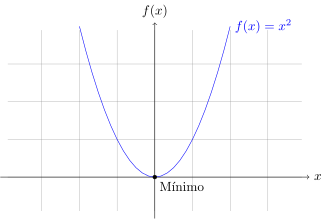
\includegraphics[keepaspectratio]{index_files/mediabag/parabolaMin.pdf}}

Outras, por sua vez, possuem máximo, mas não mínimo, como o gêmeo do mal
dessa última função: \(g(x) = -x^2\).

\pandocbounded{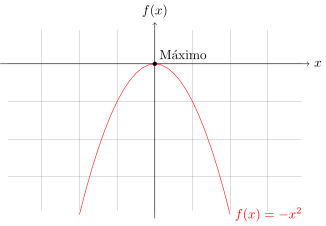
\includegraphics[keepaspectratio]{index_files/mediabag/parabolaMax.pdf}}

Outras funções, por sua vez, não gostam de se limitar: \(h(x) = x\) não
possuí máximo ou mínimo.

\pandocbounded{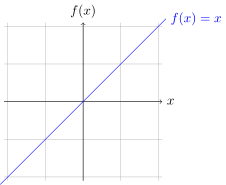
\includegraphics[keepaspectratio]{index_files/mediabag/identidade.pdf}}

Se você está bem iterado com nosso capítulo sobre o Teorema de
Weierstrass do cálculo univariado, você prontamente se lembra que, para
uma função garantidamente possuir máximo e mínimo, basta que seu domínio
seja \emph{limitado} (ou seja, não vá para mais ou menos infinito) e
\emph{fechado}. Uma consequência disso é que, caso escolhamos olhar para
uma função qualquer em um intervalo fechado de seu domínio,
conseguiremos encontrar pontos de \emph{máximo e mínimo locais}. Vamos
tomar nossa última função, \(f(x) = x\) como exemplo limitando-a ao
intervalo \([-1,1]\)

\pandocbounded{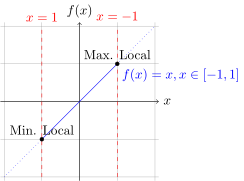
\includegraphics[keepaspectratio]{index_files/mediabag/identidadeLimitada.pdf}}

Temos uma visualização do Teorema de Weierstrass: toda função fechada e
limitada possuí ponto de máximo e mínimo.

\section{Técnicas para encontrar máximos e
mínimos}\label{tuxe9cnicas-para-encontrar-muxe1ximos-e-muxednimos}

Vamos nos lembrar da aplicação do Teorema de Weierstrass que vimos
anteriormente para encontrar máximos e mínimos.

Primeiro, podemos perceber que, nos pontos de máximo e mínimo, quando
existem, se traçarmos uma reta tangente a estes teremos quase sempre uma
reta horizontal/perpendicular ao eixo \(x\) (Verifique o último caso em
que limitamos a função identidade: isso nem sempre vale!).

\pandocbounded{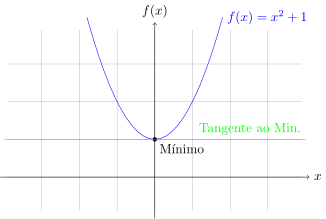
\includegraphics[keepaspectratio]{index_files/mediabag/parabolaMinTangente.pdf}}

\pandocbounded{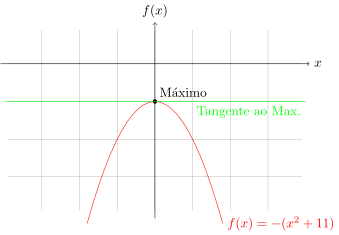
\includegraphics[keepaspectratio]{index_files/mediabag/parabolaMaxTangente.pdf}}

Podemos visualizar isso de forma analítica através da seguinte
proposição:

\emph{Proposição} Seja \(f: A\rightarrow B\) uma função diferenciável.
Se \(f(x)\) é ponto de máximo ou mínimo, \(f'(x) = 0\)

Precisamos tomar atenção com a ordem dessa implicação! Um ponto de
máximo ou mínimo de uma função diferenciável implica que a derivada
dessa função neste ponto, se existe, é sempre 0. Contudo, um ponto com
derivada 0 não necessariamente é ponto de máximo ou mínimo! Dos gráficos
acima, vimos que \((0,0)\) é o ponto de mínimo e máximo das funções
\(x^2\) e \(-x^2\), respectivamente. Vamos conferir suas derivadas:

\[
\begin{aligned}
    f(x) = x^2 \Rightarrow f'(x) = 2x \therefore f'(0) = 0~ \checkmark \\
    f(x) = -x^2 \Rightarrow f'(x) = -2x \therefore f'(0) = 0 ~\checkmark \\
\end{aligned}
\]

Mas podemos encontrar derivadas com valor 0 em determinados pontos que
não são de máximo ou mínimo!

\[
f(x) = x^3 \Rightarrow f'(x) = 3x^2 \therefore f'(x) = 0 \Rightarrow x = 0
\]

Vamos visualizar o gráfico dessa função e conferir se \((0,0)\) é ponto
de máximo ou mínimo:

\pandocbounded{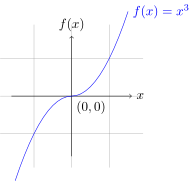
\includegraphics[keepaspectratio]{index_files/mediabag/xcuboSemMinMax.pdf}}

A derivada no ponto \(x=0\) é, de fato, \(0\) (note que a tangente é o
próprio eixo x), contudo, esse ponto não é mínimo nem máximo da função
que, por sua vez, não apresenta nenhum valor de máximo ou mínimo global.

Com isso em mente, precisaremos de mais informações para deduzirmos se
um desses pontos é ponto de máximo, mínimo ou nenhum dos dois se formos
analisar apenas as derivadas, sem o auxílio de gráficos.

Voltando para nossas parábolas, caso derivarmos novamente a primeira
função, \(f(x) = x^2\), teremos \(f'(x) = 2x\) e \(f''(x) = 2\) um valor
sempre positivo. Se você se lembra da interpretação das derivadas, isso
significa que, analisando a primeira derivada, a função é decrescente no
intervalo \((-\infty, 0)\) e crescente no intervalo \((0, \infty)\). Da
cada segunda derivada, sempre positiva, temos que a taxa de variação em
si é sempre crescente (quando decresce, decresce cada vez mais rápido e
quando cresce, cresce cada vez mais rápido). Dessa forma, como no ponto
\((0,0)\) nossa primeira derivada é 0, a função passa de decrescente
para crescente e, pela segunda derivada, a concavidade dessa parábola
está para cima. Por isso, esse ponto é o ponto de mínimo da função.

\pandocbounded{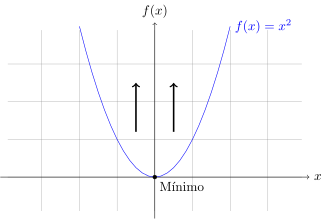
\includegraphics[keepaspectratio]{index_files/mediabag/parabolaMinSetas.pdf}}

Com a mesma lógica, usando a segunda derivada da função
\(f(x) = -2x^2, f''(x) = -2\), temos que a concavidade de nossa parábola
está para baixo.

\pandocbounded{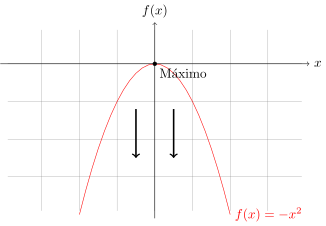
\includegraphics[keepaspectratio]{index_files/mediabag/parabolaMaxSetas.pdf}}

Complementando esses conceitos, a segunda derivada no ponto \((0,0)\) da
nossa função problemática, \(f(x) = x^4\), ainda é 0:
\(f''(x) = 6x \Rightarrow f''(0) =0\), o que não nos permite concluir se
\((0,0)\) é ponto de máximo, mínimo ou nenhum.

Portanto, podemos construir uma tabela para analisarmos máximos e
mínimos \[
\begin{array}{c|c|c|c}
    \text{Função} & f'(0) & f''(0) & (0,0) \\
    \hline
    f(x) = x^2 &  0 &  > 0 ~\forall x & \text{Mínimo} \\
    f(x) = -x^2 &  0 &  < 0 ~\forall x & \text{Máximo} \\
    f(x) = x^3 &  0 &  \in \mathbb{R} & \text{Inconclusivo} 
\end{array}
\]

\part{Aplicações do Cálculo}

\part{Álgebra Linear}

\chapter{Espaços Vetoriais}\label{espauxe7os-vetoriais}

Neste curso, poderemos contentarmo-nos com a intuição de que
\emph{``espaço vetorial''} é simplesmente o espaço onde habitam os
elementos com que faremos as nossas contas. Cada um desses elementos do
espaço vetorial receberá um nome especial: \emph{``vetor''}. Muito
provavelmente, você deve recordar-se dos vetores como aquelas
``setinhas'' que usávamos nas aulas de física para representar as forças
atuando sobre um corpo. Por sorte, compreender os vetores como uma
``setinha'' ainda é uma interpretação geométrica muito funcional para a
maior parte do curso!

\section{Exemplos de espaços
vetoriais}\label{exemplos-de-espauxe7os-vetoriais}

\begin{enumerate}
\def\labelenumi{\arabic{enumi}.}
\tightlist
\item
  O exemplo mais fundamental são os vetores usados pela física para
  representar forças
\item
  Uma rede de supermercados possui cinco filiais. Cada filial registra,
  a cada dia, o saldo ao final do dia de cada uma das suas três caixas
  registradores na forma de uma lista (\(caixa_{1}\), \(caixa_{2}\),
  \(caixa_{3}\))
\item
  A velocidade de um cometa em relação ao planeta Terra
\item
  A velocidade de quatro cometas em relação ao planeta Terra
  (\(cometa_{1}\), \(cometa_{2}\), \(cometa_{3}\), \(cometa_{4}\))
\end{enumerate}

\section{Formalizando o espaço vetorial e seus
elementos}\label{formalizando-o-espauxe7o-vetorial-e-seus-elementos}

Para os mais interessados, vamos começar fornecendo os critérios
fundamentais para um conjunto ser chamado de espaço vetorial. Não é
fundamental decorar as propriedades, leia apenas se você tiver interesse
em compreender melhor o tópico.

Um conjunto não vazio V é um espaço-vetorial sobre um corpo
\(\mathbb{K}\) (um objeto matemático em que as operações
\(+, -, \times,\div\) funcionam como nós conhecemos) se, em seus
elementos, denominados vetores, estiverem definidas a soma de vetores, a
multiplicação por escalar e valerem as seguintes oito propriedades:

Para a Adição:

(A1) \(u+v = v+u,  \forall  u,v \in V\) (propriedade comutativa)

(A2) \((u+v)+w = u+(v+w),  \forall  u,v,w \in V\) (propriedade
associativa)

(A3) existe um vetor \(v\), chamado ``vetor nulo'' e denotado \(0\), tal
que \(0+v=v, \forall v \in V\) (elemento neutro da soma)

(A4) a cada vetor \(v \in V\), existe um vetor em \(V\), denotado por
\(-v\), tal que \(v+(-v)=0\) (existência do oposto)

Para a Multiplicação por escalar (número real na maioria dos casos):

(M1)
\((\alpha \beta) \cdot v = \alpha (\beta \cdot v), \forall \alpha , \beta \in \mathbb{K} \text{ e } \forall  v \in V\)
(propriedade associativa)

(M2) \(1 \cdot v = v,  \forall v \in V\) (elemento neutro da
multiplicação)

(M3)
\(\alpha \cdot (u+v)=\alpha \cdot u + \alpha \cdot v,  \forall \alpha \in \mathbb{K} \text{ e } \forall u,v \in V\)

(M4)
\((\alpha + \beta) \cdot v = \alpha \cdot u + \beta \cdot u, \forall \alpha, \beta \in \mathbb{K} \text{ e } \forall v \in V\)

Dessa extensa definição, basta tirar a seguinte interpretação: chamamos
de vetor cada um dos elementos pertencentes ao conjunto em que estamos
definindo o espaço vetorial. Podemos somar os vetores, podemos
multiplicar os vetores por um escalar (número real) e aquelas velhas
propriedades que aprendemos na escola ainda valem: a ordem dos elementos
não afeta a soma nem a multiplicação, podemos usar parênteses para
alterar a ordem das operações e vale a propriedade distributiva.

Durante os cursos de cálculo, veremos o espaço vetorial diversas vezes,
mas trabalharemos sempre com múltiplos do conjunto dos reais
(\(\mathbb{R}\)).

\section{Vetores aplicados a
Cálculo}\label{vetores-aplicados-a-cuxe1lculo}

Ainda que seja ótimo desenvolvermos um certo rigor com a matemática, nem
sempre é necessário e pode gerar mais confusões do que entendimentos.
Desse ponto em diante, traremos o conteúdo de vetores e o espaço
vetorial da maneiras mais sucinta possível!

Considere o espaço \(R^2\). Nossa melhor maneira de representá-lo é por
meio do plano cartesiano. Cada ponto no plano cartesiano é representado
por uma dupla \((x, y)\). Por convenção, adotamos que o primeiro
elemento é sempre a coordenada \(x\) e o segundo elemento é a coordenada
\(y\). Fixe, agora, um ponto qualquer no plano, por exemplo \((3,4)\) e
construa uma seta que liga o ponto à origem \((0,0)\). Essa seta que
acabamos de criar é a representação gráfica do vetor \((3,4)\). Note que
o vetor e o ponto têm a mesma notação, isso ocorre, pois são conceitos
muito próximos e com muitas interações.

Durante seus estudos, você também pode ver os vetores representados como
\([x,y]\). Ou até mesmo verticalmente: \[
\begin{bmatrix}
  x  \\
  y 
\end{bmatrix}
\] Uma outra maneira de interpretar vetores é enxergando-os como uma
matriz de dimensão \(1 \times 2\) ou \(2 \times 1\), respectivamente.
Chamamos de vetor linha linha e vetor coluna, ainda que sejam,
conceitualmente, objetos muito próximos.

Ao utilizar vetores, é muito comum separar os seus elementos por uma
vírgula ou apenas separá-los com um espaçamento maior. Durante seus
estudos, opte por uma notação e tome cuidado para não confundir a
vírgula usada para separar os elementos com a vírgula usada para
expressar casas decimais! Para evitar a confusão, sugerimos que você
adote o ponto (.) como separador decimal ou use o ponto e vírgula (;)
para separar os elementos do vetor.

\section{Somando Vetores}\label{somando-vetores}

A soma de vetores é uma operação extremamente simples, mas segue algumas
pequenas regras: só é possível somar vetores de mesmo tamanho
(comprimento) e cada elemento do vetor resultante é igual à soma dos
correspondes. Acompanhe os exemplos:

\begin{enumerate}
\def\labelenumi{\arabic{enumi}.}
\tightlist
\item
  \((x_1, y_1) + (x_2, y_2) = (x_1+x_2 \phantom{-}
  , \phantom{-} y_1 + y_2)\)
\item
  \((x_1, y_1) - (x_2, y_2) = (x_1-x_2 \phantom{-}
  , \phantom{-} y_1 - y_2)\)
\item
  \((0,5)+(2,4)=(2,9)\)
\item
  \((0,5)-(2,4)=(-2,1)\)
\item
  \((\pi, e)+(1,2) = (\pi+1, e+2)\)
\item
  \((\pi, e)-(1,2) = (\pi-1, e-2)\)
\item
  \([1,3]+[4,-6]=[5,-3]\)
\item
  \([1,3]-[4,-6]=[-3,9]\)
\item
  \[
  \begin{bmatrix} 4  \\  8 \end{bmatrix}+
  \begin{bmatrix} 3  \\  1 \end{bmatrix}=
  \begin{bmatrix} 7  \\  9 \end{bmatrix}
  \]
\item
  \[
  \begin{bmatrix} 4  \\  8 \end{bmatrix}-
  \begin{bmatrix} 3  \\  1 \end{bmatrix}=
  \begin{bmatrix} 1  \\  7 \end{bmatrix}
  \]
\end{enumerate}

\section{Multiplicando Vetores}\label{multiplicando-vetores}

A multiplicação de vetores é uma operação muito simples e intuitiva.
Atente-se que só é possível multiplicar um vetor por um escalar
(geralmente um número real). Para efetuar a operação, basta multiplicar
cada um dos elementos do vetor pelo escalar. Lembre-se que dividir por
um número é equivalente a multiplicar pelo inverso:
\(x \div 5 = x \times \frac{1}{5}\) e que a multiplicação é comutativa,
ou seja, podemos inverter a ordem dos termos. Veja os exemplos:

\begin{enumerate}
\def\labelenumi{\arabic{enumi}.}
\tightlist
\item
  \(\lambda \times (x,y) = (x,y) \times \lambda = (x \times \lambda, y \times \lambda)\)
\item
  \((x,y) \div \lambda = (x,y) \times \frac{1}{\lambda} = \frac{1}{\lambda} \times (x,y) = (\frac{x}{\lambda}, \frac{y}{\lambda})\)
\item
  \((2,5) \times 3 = (6,15)\)
\item
  \((2,5) \div 3 = (\frac{2}{3}, \frac{5}{3})\)
\item
  \(7(0, 8) = (0,56)\)
\item
  \([10, 20] \div 5 = [2, 4]\)
\item
  \[
  \begin{bmatrix} 144  \\  96 \end{bmatrix} \div
  12=
  \begin{bmatrix} 12  \\  8 \end{bmatrix}
  \]
\item
  \[
  \begin{bmatrix} \frac{5}{7}  \\  \frac{17}{6} \end{bmatrix} \times
  \frac{3}{8} =
  \begin{bmatrix} \frac{15}{56}  \\  \frac{17}{16} \end{bmatrix}
  \]
\end{enumerate}

Note que não é possível dividir um escalar por um vetor e tampouco é
possível multiplicar ou dividir vetores entre si!

\section{Produto Interno}\label{produto-interno}

Nessa seção, introduziremos uma nova operação entre dois vetores: o
produto interno. Em um curso de álgebra linear, tal operação pode ser
definida de diversas maneiras diferentes, mas restringiremo-nos ao
``produto interno usual'', que é assim definido: \[
(x_1, y_1) \cdot (x_2, y_2) = x_1 \times x_2 + y_1 \times y_2
\]

Note que o produto interno é uma operação que recebe dois vetores de
mesmo tamanho e resulta em um número. Tal operação possui outras
notações e nomes, como ``produto escalar'', mas trata-se do mesmo
processo. \[
(x_1, y_1) \cdot (x_2, y_2) = \langle (x_1, y_1),(x_2, y_2) \rangle
\]

A notação \(\langle a,b \rangle\) é comumente usada na física, mas não é
raro ver matemáticos usando-as também.

Veja alguns exemplos: 1. \((2,4) \cdot (3,7) = 6+28=34\) 2.
\((4,2) \cdot (4,2) = 16+4 = 20\) 3. \((0,21) \cdot (13, 0) = 0+0=0\) 4.
\(\langle (4,8),(3,2) \rangle = 12+24=36\)

\subsection{Norma de um Vetor}\label{norma-de-um-vetor}

Ainda considerando o produto interno, vamos definir uma segunda operação
com um vetor: a norma. A norma de um vetor nada mais é do que a raiz
quadrado do produto interno do vetor com ele mesmo, usamos \(|| a ||\)
para representar a norma de um vetor. \[
||a|| = \sqrt{a \cdot a} = \sqrt{\langle a,a \rangle}
\] Geometricamente, entende-se a norma de um vetor como o seu
``comprimento''. Usando a nossa primeira intuição de vetores como uma
seta ligando a origem a um ponto, desenhe o vetor \((3,4)\) e calcule
seu comprimento usando o Teorema de Pitágoras. Em seguida, calcule a
norma do vetor. Se todas as contas estiverem corretas, você deve ter
concluído que tanto a norma quando o comprimento do vetor são 5.

Você deve estar familiarizado com o operador \(|a|\), que é o módulo de
\(a\). Matematicamente, define-se o módulo de um número como
\(|a| = \sqrt{a^2}\). Note que essa definição é apenas a norma de um
vetor de tamanho um, ou seja, calcular o módulo de um número nada mais é
do que calcular o seu ``tamanho'', ou o quão longe está da origem.

Acompanhe alguns exemplos do cálculo de uma norma:

\begin{enumerate}
\def\labelenumi{\arabic{enumi}.}
\tightlist
\item
  \(||(x,y)|| = \sqrt{x^2+y^2}\)
\item
  \(||(5,12)|| = \sqrt{25+144} = 13\)
\item
  \(||(24, 7)|| = \sqrt{576+49}=25\)
\item
  \(||(7,5)|| = \sqrt{49+25}=\sqrt{74}\)
\end{enumerate}

\subsection{Vetores Perpendiculares}\label{vetores-perpendiculares}

Uma característica particularmente útil do produto interno é que ele é
capaz de nos revelar quando dois vetores são ortogonais. Ainda que não
sejam equivalentes, pode-se considerar ortogonalidade como um sinônimo
de perpendicularidade, ou seja, quando o produto interno de dois vetores
é 0, eles ``formam um ângulo de \(90^{\circ}\) entre si''.

Para testar tal propriedade, desenhe no plano cartesiano os vetores
\((3,0)\) e \((0,5)\) e calcule o produto interno entre eles. Repita o
mesmo processo, num novo plano, com os vetores \((-3,4)\) e \((8,-6)\).
Você consegue encontrar mais um vetor que seja ortogonal ao vetor
\((-3,4)\)? Pegue o vetor que você encontrou e divida-o pela sua norma.
Você deve ter chegado em \((\frac{4}{5}, \frac{3}{5})\) ou
\((-\frac{4}{5}, -\frac{3}{5})\).

\subsection{Versores}\label{versores}

Durante o estudo do Cálculo, é muito comum que as formulações utilizem
versores ao invés dos usuais vetores. Por sorte, todo o conteúdo vistos
até agora nesse capítulo nos permite compreender facilmente o que é um
versor!

\emph{Define-se o versos como um vetor unitário que tem mesma direção e
sentido que outro vetor.}

Ou seja, um versor de um vetor é uma versão daquele mesmo vetor, mas com
norma igual a \(1\).

Utilizaremos \(\hat{a}\) para denotar um versor. \[
\hat{a}=\frac{a}{||a||}
\] Alguns exemplos de versores:

\begin{enumerate}
\def\labelenumi{\arabic{enumi}.}
\tightlist
\item
  \(a = (6,8) \rightarrow \hat{a} = \frac{(6,8)}{||(6,8)||}=\frac{(6,8)}{10} = (\frac{3}{5}, \frac{4}{5})\)
\item
  \(a = (4,2) \rightarrow \hat{a} = \frac{(4,2)}{||(4,2)||}=\frac{(4,2)}{\sqrt{20}} = (\frac{4}{\sqrt{20}},
   \frac{2}{\sqrt{20}})=(\frac{\sqrt{20}}{5}, \frac{\sqrt{20}}{10})\)
\end{enumerate}

Em um plano cartesiano, desenhe o vetor \((-6,8)\), calcule sua norma,
desenhe o seu versos e, por fim, desenhe um círculo de raio \(1\)
centrado na origem. Você verá uma das muitas belezas dos vetores. Tente
repetir este processo com outros vetores, todos terão a mesma
propriedade que você acabou de visualizar. Tente provar esse resultado!

\part{Cálculo Multivariado}

\chapter{Curvas}\label{curvas}

Um dos principais objetos matemáticos no estudo de cálculo são as
\emph{curvas}, funções contínuas que mapeiam intervalos dos números
reais para espaços vetoriais, como
\(\mathbb{R}^2, \mathbb{R}^3,\ldots,\mathbb{R}^n\), ou seja, para um
intervalo \(I\), dos reais, uma curva é tal que
\(\gamma : I \rightarrow \mathbb{R}^n\). Dessa forma, seu domínio é o
próprio intervalo \(I\), seu contradomínio é \(\mathbb{R}^n\) e sua
imagem é o conjunto \(\{\gamma(t) \in \mathbb{R}^n : t \in I\}\). Essa
imagem, também chamada de trajetória de \(\gamma\), é o lugar geométrico
descrito como o resultado dessa função conforme t varia por seu domínio.

um exemplo de uma simples curva parametrizada por \(t\): \[
\begin{aligned}
    \gamma(t) = (t, -t) \Rightarrow \gamma(1) = (1, -1); \gamma(0) = (0,0). \\ 
    \mathrm{Imagem}\gamma = \mathrm{Im}\gamma =
    \text{ reta de equações paramétricas } 
    \begin{cases}
        x = t \\
        y = -t
    \end{cases}
\end{aligned}
\]

Dessa forma, vimos que curvas podem ser coisas muito simples, como a
reta acima, ou figuras mais complexas, como parábolas
\(\gamma(t) = (t, t^2 + t + 1)\), circunferências
\(\gamma(t) = (\cos(t),\mathrm{sin}(t)), t \in [0, 2\pi]\) ou até
espirais, como nosso DNA, \(\gamma(t) = (t, \cos(t), \mathrm{sin}(t))\)
(note que esse é 3d! podemos escolher qualquer dimensão para nossas
curvas).

\section{Domínio de uma curva}\label{domuxednio-de-uma-curva}

Ao criarmos curvas, precisamos nos atentar ao seu domínio. Uma curva
parametrizada por \(t\) deve ter seus \(t\)s num intervalo que faça
sentido para sua forma. Por exemplo, em uma curva como
\(\gamma : I \rightarrow \mathbb{R}^2, \gamma(t) = (-t, \sqrt(2))\), t
só pode assumir valores positivos por seu contradomínio ser um vetor de
números reais (\(\mathbb{R}^2\)) e não os números complexos
\(\mathbb{C}\). Dessa forma, podemos descrever o domínio de \(\gamma\)
como \(\mathbb{R}^{+}\), os números reais positivos.

As vezes precisamos ser ainda mais precisos. Considere a curva
\(\gamma : I \rightarrow \mathbb{R}^2, \gamma(t) = \left(t^2, \frac{1}{t-2}\right)\).
Com algum cuidado, percebemos rapidamente que essa função não estaria
definida para \(t = 2\) (por quê?). Sendo assim, seu domínio, \(I\),
pode ser descrito como \(\mathbb{R} \setminus \{2\}\), ou seja, todo o
conjunto de números reais \emph{exceto} o número 2.

\section{Operações numa curva}\label{operauxe7uxf5es-numa-curva}

Curvas comportam-se similarmente à funções que conhecemos. Podemos
multiplicá-los por valores reais \[
\lambda \in \mathbb{R}, (\lambda\gamma)(t) = \lambda\gamma(t)
\]

Podemos somá-las \[
(\gamma_{1} + \gamma_{2})(t) = \gamma_{1}(t) + \gamma_{2}(t); 
\]

Podemos multiplicá-las por funções com contradomínio nos reais e de
mesmo domínio, (chamadas funções escalares,
\(f : I \rightarrow \mathbb{R}\), são as funções que conhecemos e
trabalhamos em cáculo univariado). \[
(f\gamma)(t) = f(t)\gamma(t)
\]

Podemos também obter o \emph{produto escalar} entre duas curvas como
vimos em nosso estudo de espaços vetoriais \[
(\gamma_{1} \cdot \gamma_{2})(t) = \gamma_{1}(t) \cdot \gamma_{2}(t)
\]

\textbf{Exercício} Dado as curvas
\(gamma_{1} = (t, 7 - t), \gamma_{2} = \left(\frac{t}{3}, t^2\right)\),
a função escalar \(f(t) = \mathrm{e}^t\) e uma constante real
\(\lambda = 2\pi\), verifique as propriedades acima. Você consegue
esboçar os gráficos da imagem de \(\gamma_{1}\) e \(\gamma_{2}\)?

\section{Continuidade e limites de
curvas}\label{continuidade-e-limites-de-curvas}

Ao tomarmos um limite de uma curva num ponto a,
\(\lim_{t\rightarrow a} \gamma(t)\), pode ser avaliado como o limite de
cada componente do vetor da imagem. Ou seja, para uma curva como
\(\gamma(t) = \left(\frac{\mathrm{sen}(t)}{t}, \frac{1}{\ln{t}}\right)\)
temos \[
\lim_{t\rightarrow 0}\gamma(t) = \left(\lim_{t\rightarrow 0} \frac{\mathrm{sen}(t)}{t}, 
\lim_{t\rightarrow 0} \frac{1}{\ln{t}}\right)  = (1, 0)
\]

Dessa forma, assim como as funções univariadas que estamos acostumados,
uma curva é contínua em determinado ponto se existe o limite dela nesse
ponto.

\section{Derivadas e integrais}\label{derivadas-e-integrais}

Para os atenciosos, reconhecer que podemos tirar o limite de uma curva
em determinado ponto já soa um sinal. Podemos encontrar as derivadas?
Vamos tentar aplicar a definição da derivada univariada em a de uma
curva \(\gamma(t) = (t^2, t)\) \[''
\lim_{t\rightarrow a} \frac{\gamma(t)-\gamma(a)}{t-a}
\]

Chamando os componentes de \(\gamma(t)\) de \(f_{1}(t)\) e \(f_{2}(t)\),
podemos aplicar o que vimos anteriormente dos limites para passar a
derivada ``para o lado de dentro'' \[
\lim_{t\rightarrow a} \frac{\gamma(t) - \gamma(a)}{t-a} = \left(\lim_{t \rightarrow a} \frac{f_{1}(t) - f_{1}(a)}{t-a},
\lim_{t \rightarrow a}\frac{f_{2}(t)-f_{2}(a}{t-a} \right) = (2a, 1)
\]

Concluímos que \(\gamma(t)' = (f_{1}(t)', f_{2}(t)')\).

Com o mesmo raciocínio, podemos integrar curvas \[
\int_{a}^{b} \gamma(t)dt = \left(\int_{a}^{b} f_{1}(t)dt, \int_{a}^{b}f_{2}(t)dt\right)
\]

\subsection{Comprimento de curvas}\label{comprimento-de-curvas}

\[
L(\gamma) = \int^{a}_{b} \lVert \gamma'(t) \rVert dt
\]

\chapter{Limites de mais de uma
variável}\label{limites-de-mais-de-uma-variuxe1vel}

Quando estudamos os \href{limites.qmd}{limites no cálculo univariado},
vimos a importância deste conceito para além de seu papel fundamental na
construção formal do cáculo. Isto é, estudamos como são importantes no
estudo do mundo natural, como na física e química, e até mesmo nas
humanidades, como na economia.

Entretanto, poucas coisas na realidade comportam-se apenas com uma única
variável. Por isso, precisamos estender o conceito de limites para
funções multivariadas, e esse será o objetivo desse capítulo.

\section{Outras formas de dividirmos o
domínio}\label{outras-formas-de-dividirmos-o-domuxednio}

No cálculo de uma variável, costumamos dividir o domínio em duas partes,
``à esquerda'' com \(\{x: x < a\}\) e ``à direita'' com
\(\{x : x > a \}\). Contudo, poderíamos também dividir o domínio de
outras formas. Vamos trabalhar um exemplo

\[
f(x) = \begin{cases}
\sqrt{2}x, x \in \mathbb{Q} \\
x^2, x \in \mathbb{R} \setminus \mathbb{Q}
\end{cases}
\]

\emph{Nota:} \(\mathbb{R} \setminus \mathbb{Q}\) significa o conjunto
que contém todos os números reais que não são racionais

podemos expressar os limites de \(x\) se aproximando de um valor
arbitrário \(a\) como \[
\begin{aligned}
\lim_{\begin{aligned}x&\rightarrow a \\ x& \in\mathbb{Q}\end{aligned}} f(x) =
\lim_{\begin{aligned}x&\rightarrow a \\ x& \in\mathbb{Q}\end{aligned}} \sqrt{2} x=
\sqrt{2} a \\
\lim_{\begin{aligned}x&\rightarrow a \\ x& \in \mathbb{R}\setminus\mathbb{Q}
\end{aligned}} f(x) =
\lim_{\begin{aligned}x&\rightarrow a \\ x& \in\mathbb{R}\setminus\mathbb{Q}
\end{aligned}} x^2 = a^2
\end{aligned}
\]

Dividindo o domínio em pedaços, temos que \[
\lim_{x\rightarrow a} f(x) = L \Leftrightarrow
\lim_{\begin{aligned}x&\rightarrow a \\ x& \in\mathbb{R}\setminus\mathbb{Q}
\end{aligned}} f(x) = L = 
\lim_{\begin{aligned}x&\rightarrow a \\ x& \in\mathbb{Q}\end{aligned}}
\]

Para que a igualdade à direita exista, necessitamos que
\(\sqrt{2}a = a^2\). Assim, a iguldade vale para \(a=0\) e
\(a=\sqrt{2}\). Logo, \(\lim_{x\rightarrow a} f(x)\) existe somente para
\(a=0\) e \(a=\sqrt{2}\)! Isso significa que a função é contínua apenas
em \(0\) (onde assume o valor de 0) e em \(\sqrt{2}\) (onde assume o
valor de 2).

Essa técnica de dividir o domínio é muito importante para calcularmos
limites de várias variáveis. Vamos fazer um exemplo

\subsection{Calculando limites com duas
variáveis}\label{calculando-limites-com-duas-variuxe1veis}

Temos uma função simpels, \(f(x) = \frac{x^3y^6}{x^4+y^8}\). Note que
essa função só existe quando \(x\) e \(y\) são \emph{ambos} diferentes
de 0. Mas, se quisermos descobrir o que acontece na região do
\(\mathbb{R}^2\) próxima do ponto \((0,0)\), podemos calcular o seguinte
limite:

\[
\lim_{(x,y) \rightarrow (0,0)} \frac{x^3y^6}{x^4+y^8}
\]

Vamos utilizar a técnica anterior e dividir o domínio. Para isso,
precisamos buscar uma relação entre \(\lvert x \rvert\) e
\(\lvert y \rvert\). Tentaremos encontrar \(\alpha > 0\) tal que
\(\lvert x \rvert \leq \lvert y \rvert^\alpha\) e
\(\lvert x \rvert \geq \lvert y \rvert^{\alpha} \Leftrightarrow \lvert y \rvert \leq \lvert x \rvert^{\frac{1}{\alpha}}\)

\subsubsection{Exemplo 1}\label{exemplo-1}

\begin{enumerate}
\def\labelenumi{\arabic{enumi}.}
\tightlist
\item
  \(\lvert x \rvert \leq \lvert y \rvert^{\alpha}\) \[
  0 \leq \left\lvert \frac{x^3y^6}{x^4+y^8} \right\rvert = \frac{\lvert x \rvert^3 \lvert y \rvert^6}
  {x^4+y^8} \leq \frac{\lvert y \rvert ^{3\alpha} \lvert y \rvert^6}{x^4 + y^8} =
  \frac{\lvert y \rvert^{6+3\alpha}}{x^4 + y^8}
  \]
\end{enumerate}

Se \(6+3\alpha > 8\), temos

\[
\cancelto{0}{\lvert y \rvert^{6+3\alpha-8}} \cdot
\underbrace{\frac{\lvert y \rvert^{8}}{x^4+y^8}}_{\text{Limitado}}
\]

Assim, se \(6+3\alpha > 8\), pelo \hyperref[sec-confronto]{teorema do
confronto}

\[
\lim_{\begin{aligned}(x,y)&\rightarrow (0,0) 
\\ \lvert x \rvert &\leq \lvert y \rvert^{\alpha} \end{aligned}} 
\left\lvert \frac{x^3 y^6}{x^4+y^8} \right\rvert = 0 
\]

Portanto,

\[
\lim_{\begin{aligned}(x,y)&\rightarrow (0,0) 
\\ \lvert x \rvert &\leq \lvert y \rvert^{\alpha} \end{aligned}} 
\frac{x^3 y^6}{x^4+y^8} = 0
\]

\begin{enumerate}
\def\labelenumi{\arabic{enumi}.}
\setcounter{enumi}{1}
\tightlist
\item
  \(\lvert x \rvert \geq \lvert y \rvert^{\alpha} \Leftrightarrow \lvert y \rvert \leq \lvert x \rvert^{\frac{1}{\alpha}}\)
\end{enumerate}

\[
0 \leq \left\lvert \frac{x^3y^6}{x^4+y^8} \right\rvert = 
\frac{\lvert x \rvert^3 \lvert y \rvert^6}{x^4+y^8} \leq
\frac{\lvert x \rvert^3 \lvert x \rvert^{\frac{6}{\alpha}}}{x^4+y^8}
\]

Se \(3 + \frac{6}{\alpha} > 4\), então \[
\leq \frac{\lvert x \rvert^{3 \frac{6}{\alpha}}}{x^4+y^8} =
\cancelto{0}{\lvert x \rvert^{3 + \frac{6}{\alpha} - 4}} \cdot
\underbrace{\frac{\lvert x \rvert^4}{x^4+y^8}}_{\text{Limitado}}
\]

Para \(3 + \frac{6}{\alpha} > 4\) temos pelo
\href{limites.qmd$sec-confronto}{teorema do confronto},

\[
\lim_{\begin{aligned}(x,y)&\rightarrow (0,0) \\ 
\lvert x \rvert & \geq \lvert y \rvert^{\alpha} \end{aligned}}
\left\lvert \frac{x^3y^6}{x^4+y^8} \right\rvert = 0
\]

Portanto,

\[
\lim_{\begin{aligned}(x,y)&\rightarrow (0,0) \\ 
\lvert x \rvert & \geq \lvert y \rvert^{\alpha} \end{aligned}}
\frac{x^3y^6}{x^4+y^8}  = 0
\]

Vamos analisar esse número \(\alpha\). Sabemos pelo ponto 1. que
\(6 + 3\alpha - 8 >0\) e pelo ponto 2. que
\(3 + \frac{6}{\alpha} - 4 >0\).

\[
1. ~~~
\begin{aligned}
  &6 + 3\alpha - 8 > 0 \\
  &\Leftrightarrow 3\alpha > 2 \\
  &\Leftrightarrow \alpha > \frac{2}{3} \\
\end{aligned} ~~~~~~~~
2. ~~~
\begin{aligned}
  &3 + \frac{6}{\alpha} > 4 \\
  &\Leftrightarrow \frac{6}{\alpha} > 1 \\
  &\Leftrightarrow \alpha < 6
\end{aligned}
\]

Dessa forma, para termos os dois limites nessa repartição, vasta
considerar \(\alpha\) com \(\frac{2}{3}<\alpha<6\). Podemos, por exempo,
tomar \(\alpha = 1\). Com isso,

\[
\lim_{\begin{aligned}
(x,y)&\rightarrow(0,0)\\ \lvert x \rvert &\leq \lvert y \rvert
\end{aligned}}
\frac{x^3y^6}{x^4+y^8} = 0 =
\lim_{\begin{aligned}
(x,y)&\rightarrow(0,0)\\ \lvert x \rvert &\geq \lvert y \rvert
\end{aligned}}
\frac{x^3y^6}{x^4+y^8}
\]

Assim, calculamos nosso limite após dividí-lo em relação ao módulo de
\(x\) e \(y\) e obtermos um mesmo valor \(L=0\)

\[
\lim_{(x,y)\rightarrow(0,0)}
\frac{x^3y^6}{x^4+y^8} = 0
\]

\subsubsection{Exemplo 2}\label{exemplo-2}

\[
\lim_{(x,y)\rightarrow (0,0)} \frac{x^3y^3}{x^4+y^8}
\]

Tentaremos novamente dividir o domínio através de uma relação entre o
módulo de \(x\) e o módulo de \(y\). Isto é, vamos tentar encontrar
\(\alpha>0\) tal que \(\lvert x \rvert \leq \lvert y \rvert^{\alpha}\) e
\(\lvert x \rvert \geq \lvert y \rvert^{\alpha}\)

\begin{enumerate}
\def\labelenumi{\arabic{enumi}.}
\tightlist
\item
  \(\lvert x \rvert \leq \lvert y \rvert^{\alpha}\)
\end{enumerate}

\[
0 \leq \left\lvert \frac{x^3y^3}{x^4+y^8}\right\rvert
\leq \frac{\lvert y \rvert^{3\alpha}\lvert y \rvert^{3}}{x^4+y^8}
\]

Se \(3 \alpha + 3 > 8\)

\[
= \cancelto{0}{\lvert y \rvert ^{3\alpha + 3 - 8}} \cdot
\underbrace{\frac{\lvert y \rvert^8}{x^4+y^8}}_{\text{Limitado}} = 0
\]

Se \(3 \alpha + 3 > 8\), então pelo
\href{limites.qmd$sec-confronto}{teorema do confronto},

\[
\lim_{\begin{aligned}(x,y)\rightarrow (0,0)
\\ \lvert x \rvert \leq \lvert y \rvert^{\alpha}
\end{aligned}} \left\lvert \frac{x^3y^3}{x^4+y^8} \right\rvert = 0
\]

Logo, \[
\lim_{\begin{aligned}(x,y)\rightarrow (0,0)
\\ \lvert x \rvert \leq \lvert y \rvert^{\alpha}
\end{aligned}} \frac{x^3y^3}{x^4+y^8} = 0
\]

\begin{enumerate}
\def\labelenumi{\arabic{enumi}.}
\setcounter{enumi}{1}
\tightlist
\item
  \(\lvert x \rvert \geq \lvert y \rvert^{\alpha}\), o que é equivalente
  a \(\lvert y \rvert \leq \lvert x \rvert^{\frac{1}{\alpha}}\)
\end{enumerate}

\[
0 \leq \left\lvert \frac{x^3y^3}{x^4+y^8}\right\rvert = 
\frac{\lvert x \rvert^3 \lvert y \rvert^3}{x^4+y^8}
\leq \frac{\lvert x \rvert^3 \lvert x \rvert^{\frac{3}{\alpha}}}{x^4+y^8}
\]

Se \(3 + \frac{3}{\alpha} > 4\), temos

\[
= \cancelto{0}{\lvert x \rvert^{3+ \frac{3}{\alpha}-4}} \cdot
\underbrace{\frac{\lvert x \rvert^4}{x^4+y^8}}_{\text{Limitado}} = 0
\]

Assim, se \(3 + \frac{3}{\alpha} > 4\), então pelo
\href{limites.qmd$sec-confronto}{teorema do confronto},

\[
\lim_{\begin{aligned}(x,y)\rightarrow (0,0)
\\ \lvert x \rvert \geq \lvert y \rvert^{\alpha}
\end{aligned}} \frac{x^3y^3}{x^4+y^8} = 0
\]

\[
1. ~~~
\begin{aligned}
  &3 + 3\alpha - 8 > 0 \\
  &\Leftrightarrow 3\alpha > 5 \\
  &\Leftrightarrow \alpha > \frac{5}{3} \\
\end{aligned} ~~~~~~~~
2. ~~~
\begin{aligned}
  &3 + \frac{3}{\alpha} > 4 \\
  &\Leftrightarrow \frac{3}{\alpha} > 1 \\
  &\Leftrightarrow \alpha < 3
\end{aligned}
\]

Como \(3 > \frac{5}{3}\), podemos fixar um \(\alpha\) tal que \[
\frac{5}{3} < \alpha < 3
\]

Vamos usar, por exemplo, \(\alpha = 2\). Assim,

\[
\lim_{\begin{aligned}(x,y)\rightarrow (0,0)
\\ \lvert x \rvert \leq \lvert y \rvert^{2}
\end{aligned}} \frac{x^3y^3}{x^4+y^8} = 0 = 
\lim_{\begin{aligned}(x,y)\rightarrow (0,0)
\\ \lvert x \rvert \geq \lvert y \rvert^{2}
\end{aligned}} \frac{x^3y^3}{x^4+y^8}
\]

\subsubsection{Exemplo 3}\label{exemplo-3}

\[
\lim_{(x,y)\rightarrow(0,0)} \frac{x^3y^2}{x^4+y^8}
\]

\begin{enumerate}
\def\labelenumi{\arabic{enumi}.}
\tightlist
\item
  \(\lvert x \rvert \leq \lvert y \rvert^{\alpha}\)
\end{enumerate}

\[
0 \leq \left\lvert\frac{x^3 y^2}{x^4+y^8} \right\rvert=
\frac{\lvert x \rvert^3 \lvert y \rvert^2}{x^4+y^8} \leq
\frac{\lvert y \rvert^{3\alpha} \lvert y \rvert^2}{x^4+y^8} \\
\]

Se \(3\alpha + 2 > 8\),

\[
\leq \cancelto{0}{\lvert y \rvert^{3\alpha+2-8}}
\underbrace{\frac{\lvert y \rvert^{8}}{x^4+y^8}}_{\text{Limitado}} = 0
\]

Para \(3\alpha + 2 > 8\), pelo teorema do confronto, temos \[
\lim_{\begin{aligned}(x,y)&\rightarrow (0,0) \\ 
\lvert x \rvert & \leq \lvert y \rvert^{\alpha} \end{aligned}}
\left\lvert \frac{x^3y^2}{x^4+y^8} \right\rvert = 0 \Rightarrow
\lim_{\begin{aligned}(x,y)&\rightarrow (0,0) \\ 
\lvert x \rvert & \leq \lvert y \rvert^{\alpha} \end{aligned}}
\frac{x^3y^2}{x^4+y^8} = 0
\]

\begin{enumerate}
\def\labelenumi{\arabic{enumi}.}
\setcounter{enumi}{1}
\tightlist
\item
  \(\lvert x \rvert \geq \lvert y \rvert^{\alpha} \Leftrightarrow \lvert y \rvert \leq \lvert x \rvert^{\frac{1}{\alpha}}\)
\end{enumerate}

\[
0 \leq \left\lvert\frac{x^3y^2}{x^4+y^8} \right\rvert=
\frac{\lvert x \rvert^3 \lvert y \rvert^2}{x^4+y^8} \leq
\frac{\lvert x \rvert^{3} \lvert x \rvert^{\frac{2}{\alpha}}}{x^4+y^8} \\
\]

Se \(3 + \frac{2}{\alpha} > 4\),

\[
\leq \cancelto{0}{\lvert x \rvert^{3+\frac{2}{\alpha}-4}}
\underbrace{\frac{\lvert x \rvert^{4}}{x^4+y^8}}_{\text{Limitado}} = 0
\]

Para \(3 + \frac{2}{\alpha}\) temos pelo teorema do confronto,

\[
\lim_{\begin{aligned}(x,y)&\rightarrow (0,0) \\ 
\lvert x \rvert & \geq \lvert y \rvert^{\alpha} \end{aligned}}
\left\lvert \frac{x^3y^2}{x^4+y^8} \right\rvert = 0 \Rightarrow
\lim_{\begin{aligned}(x,y)&\rightarrow (0,0) \\ 
\lvert x \rvert & \geq \lvert y \rvert^{\alpha} \end{aligned}}
\frac{x^3y^2}{x^4+y^8} = 0
\]

\[
1. ~~~
\begin{aligned}
  &3\alpha + 2 > 8 \\
  &\Leftrightarrow 3\alpha > 6 \\
  &\Leftrightarrow \alpha > 2 \\
\end{aligned} ~~~~~~~~
2. ~~~
\begin{aligned}
  &3 + \frac{2}{\alpha} > 4 \\
  &\Leftrightarrow \frac{2}{\alpha} > 1 \\
  &\Leftrightarrow \alpha < 2
\end{aligned}
\]

Como não existe um número \(\alpha\) tal que \(2 < \alpha < 2\), não
podemos usar essa estratégia para concluir se o limite existe e falhamos
em satisfazer as desigualdades para \(\alpha = 2\)

Vamos tentar outra estratégia usando \(x = y^2\), parametrizando uma
curva \(\gamma(t)=(t^2,t) \Rightarrow \gamma(0) = (0,0)\)

\[
\lim_{t\rightarrow 0} f \circ \gamma (t) = \lim_{t\rightarrow 0}
\frac{t^6 t^2}{t^8 + t^8} = \lim_{t\rightarrow 0} \frac{t^8}{2t^8} = \frac{1}{2}
\]

Vamos testar outra curva e conferir se temos um resultado único entre
elas \(\phi(t) = (0,t) \Rightarrow \phi(0) = (0,0)\)

\[
\lim_{t\rightarrow 0} f \circ \phi (t) = \lim_{t\rightarrow 0} \frac{0^3 t^2}{0^4+t^8} = 0
\]

Como
\(\lim_{t\rightarrow 0} f \circ \gamma (t) \neq \lim_{t\rightarrow 0} f \circ \phi(t)\),
segue que esse \(\lim_{(x,y)\rightarrow (0,0)} f(x,y)\) não existe.

Note que essa estratégia é útil para demonstrar que certos limites não
existem, mas caso o limite exista, teríamos que testar infinitas curvas
para provar sua existência?

\subsubsection{Exemplo 4}\label{exemplo-4}

\[
\lim_{(x,y) \rightarrow (0,0)} \frac{x^3 y^2}{x-y}
\]

Neste exemplo temos que o denominador zera num conjunto que se acumula
em (0,0). Assim para mostrar que o limite não existe, vamos nos
aproximar rapidamente do conjunto \(\{(x,y):x-y =0\}\). Para que o
denominador vá para \(0\) mais rápido do que o numerador.

Uma parametrização desse conjunto pode ser dada por \((t,t)\). Como não
queremos ``andar'' sobre \(\{(x,y):x-y =0\}\), tomaremos
\(\gamma_n (t) = (t+t^n,t)\), assim o denominador vai rapido para 0
dependendo de \(n\), pois \(t+t^n-t = t^n\).

Para isto, \(n>0\), então

\[
\begin{aligned}
\lim_{t\rightarrow 0} f \circ \gamma_{n}(t) &= \lim_{t\rightarrow 0}
\frac{(t+t^n)^3t^2}{t+t^n-t} \\
\lim_{t\rightarrow 0} \frac{t^3 (1+t^{n-3})t^2}{t^n}
\lim_{t\rightarrow 0} \frac{t^5 (1+t^{n-3})}{t^n}
\lim_{t\rightarrow 0} \frac{(1+t^{n-3})}{t^{n-5}}
\end{aligned}
\]

Pelo nuemrador, vemos que precisamos de \(n\geq 3\). Pelo denominador,
precisamos de \(n \geq 5\).

\[
\lim_{t\rightarrow 0} f\circ \gamma_5 (t) = \lim_{t\rightarrow 0} \frac{1+t^2}{1} = 1
\]

\[
\lim_{t\rightarrow 0} f\circ \gamma_6 (t) = \lim_{t\rightarrow 0} \frac{1+t^3}{t} = +\infty
\]

assim, como esses limites são diferentes, não existe \[
\lim_{(x,y)\rightarrow(0,0)} f(x,y)
\]

Neste exercício, observamos um potencial ponto falho que abriria um
caminho para mostrar que o limite não existe (nesse caso, o
denominador), e utilizamos uma estratégia para encontrar curvas que
demonstrassem isso.

\subsubsection{Exemplo 5}\label{exemplo-5}

\[
\lim_{(x,y)\rightarrow(0,0)} \frac{x^4 y^9}{x^2-y^5} = f(x,y)
\]

\((t^\frac{1}{2}, t^{\frac{1}{5}}), t > 0\) parametriza
\(\{(x,y):x^2-y^5=0, x>0, y>0\}\)

Vamos usar
\(\gamma_n(t) = \left((t+t^n)^{\frac{1}{2}}, t^{\frac{1}{5}}\right), \gamma_n(0) = (0,0)\)
novamente com a ideia de manter um denominador que fica pequeno
dependendo de \(n\) atraveś de
\(((t+t^n)^{\frac{1}{2}})^2 - (t^{\frac{1}{5}})^5 = t+t^n -t = t^n\).

\[
\begin{aligned}
\lim_{t\rightarrow 0} f \circ \gamma_n(t) &= \lim_{t\rightarrow 0}
\frac{\left((t+t^n)^{\frac{1}{2}}\right)^4 (t^\frac{1}{5})^9}{t^n} \\
& = \lim_{t\rightarrow 0} \frac{(t+t^n)^2 t^{\frac{9}{5}}}{t^n} \\
& = \lim_{t\rightarrow 0} \frac{t^2 (1+t^{n-1})^2 t^{\frac{9}{5}}}{t^n} \\
& = \lim_{t\rightarrow 0} \frac{(1+t^{n-1})^2}{t^{n-2-\frac{9}{5}}}
\end{aligned}
\]

Pelo numerador, precisamos de \(n \geq 1\). pelo denominador, precisamos
de \(n \geq \frac{19}{5}\). Vamos usar \(n = 4\),

\[
\lim_{t\rightarrow 0^{+}} f \circ \gamma_4(t) = \lim_{t\rightarrow 0^{+}}
\frac{(1+t^3)^2}{t^{4-\frac{19}{5}}} = +\infty
\]

Vamos usar outra curva para verificar o limite:
\(\phi(t) = (t,0) \Rightarrow \phi(0) = (0,0)\)

\[
\lim_{t\rightarrow 0} f \circ \phi (t) = \lim_{t \rightarrow 0} \frac{t^4 0^9}{0^2 -t^5} 
= \lim_{t\rightarrow 0} \frac{0}{-t^5} = 0
\]

Assim,
\(\lim_{t\rightarrow 0} f \circ \gamma_4(t) \neq \lim_{t\rightarrow 0} f \circ \phi (t)\).

Portanto, \(\lim_{(x,y) \rightarrow (0,0)} f(x,y)\) não existe.

\chapter{Derivadas em múltiplas
dimensões}\label{derivadas-em-muxfaltiplas-dimensuxf5es}

Quando tratamos de \href{d-simples.qmd}{derivadas} simples no cálculo
univariado, estávamos, como o nome indica, sempre tratando de funções
com uma variável. Isto é, a função estava sempre presa a um plano, e era
fácil para nós encontrarmos a reta tangente a qualquer um de seus
pontos, caso existisse, pela sua derivada.

Contudo, essas funções agora tem muito mais liberdade no cálculo
multivariado. No espaço tridimensional que vivemos, por exemplo, as
funções podem tomar formas muito além de simples curvas e retas num
plano. Sendo assim, não podemos encontrar apenas uma reta tangente a
algum ponto dessa função. Na verdade, se diferenciável, podemos
encontrar \emph{infinitas} retas tangentes num ponto, uma vez que, em
funções desse tipo, pontos possuem um \emph{plano tangente}:

\begin{figure}[H]

{\centering \pandocbounded{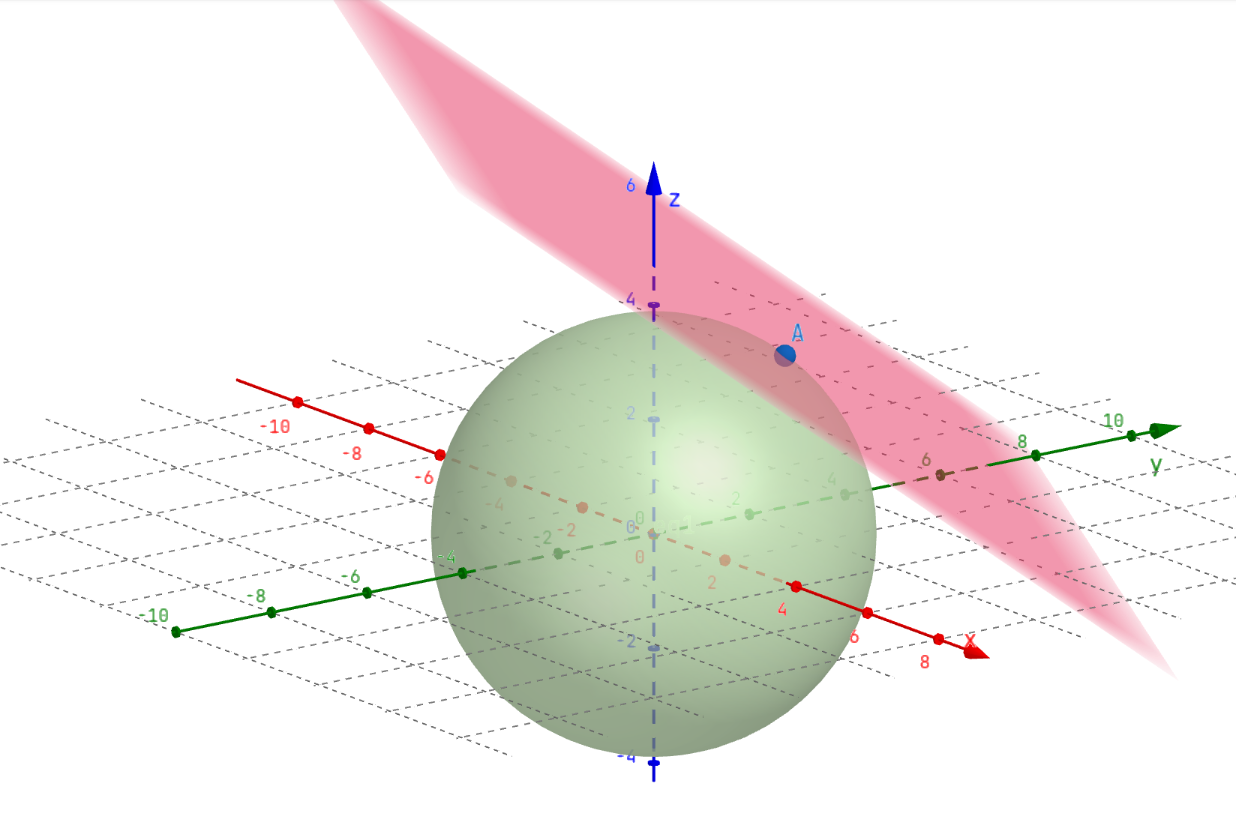
\includegraphics[keepaspectratio]{Imagens/esferaPlanoTangente.png}}

}

\caption{Plano tangente à esfera}

\end{figure}%

Observe que o plano representa todas as retas tangentes ao ponto A.

Dessa forma, diferente de como pensamos no cálculo univariado, agora as
derivadas não representam um coeficiente angular duma reta tangente, mas
sim nos dão informações sobre o plano tangente ao ponto.

\section{Derivadas Direcionais}\label{derivadas-direcionais}

Uma das formas de usar essa informação é através da \emph{derivada
direcional}. De maneira bem simples, como agora temos infinitas retas
tangentes a um ponto, podemos escolher uma direção e observar a derivada
das retas nessa direção. Isso nada mais é que analisar a derivada na
direção do vetor diretor dessas retas.

Vamos nos lembrar da definição de derivada de uma função \(f\) num ponto
\(x\) no cálculo univariado: \[
f'(x) = \lim_{h\rightarrow 0} \frac{f(x+h)-f(x)}{h}
\]

Essa definição se estende para mais dimensões ao escolhermos uma direção
para avaliar essa derivada. Chamaremos essa direção de \(y\), um vetor.
Temos assim derivada duma função \(f\) na direção de \(y\) do
\emph{ponto} \(x\) \[
f'(\pmb{x};\pmb{y}) = \lim_{h\rightarrow 0} \frac{f(\pmb{x}+h\pmb{y})-f(\pmb{x})}{h} 
\]

Temos quase a definição de nossa derivada parcial, mas ainda existe um
problema na nossa fórmula acima: por mais que ela meça a taxa de
variação de \(\pmb{x}\) na direção do vetor \(\pmb{y}\), ela não nos dá
necessariamente, em termos de escala, uma boa medida.

Isso acontece pois o vetor \(\pmb{y}\) pode não ser unitário, ou seja,
sua \emph{norma}, \(\lVert \pmb{y} \rVert\) pode ser diferente de 1.
Dessa forma, nos convém sempre normalizar o vetor que direciona esse
tipo de derivada. Vamos chamar esse \(\pmb{y}\) normado de \(\pmb{v}\),
também conhecido como \emph{versor} de \(\pmb{y}\): \[
\pmb{v} = \frac{\pmb{y}}{\lVert \pmb{y} \rVert} \Rightarrow \lVert \pmb{v} \rVert = 1
\]

Com isso, temos a definição da derivada direcional de \(f\) no ponto
\(\pmb{p}\) na direção do versor \(\pmb{v}\) de \(\pmb{y}\), denotada
por \(D_{\pmb{v}}\rvert_{\pmb{p}}\) \[
f'(\pmb{p};\pmb{v})= D_{\pmb{v}}\rvert_{\pmb{p}} = \lim_{h\rightarrow 0} \frac{f(\pmb{p}+h\pmb{v})-f(\pmb{p})}{h} 
\]

Vamos botá-la em prática!

\subsection{Exercício - Derivada
direcional}\label{exercuxedcio---derivada-direcional}

Calcule a derivada parcial de \(f(x,y) = xy\) no ponto
\(\pmb{p} = (2,1)\) na direção do vetor \(\pmb{u} = (1,1)\).

Primeiro note que o vetor \(\pmb{u}\) não possui norma 1:
\(\sqrt{1^2+1^2}=\sqrt{2}\neq 1\). Podemos norma-lo ao dividi-lo pelo
valor que acabamos de calcular:
\(\pmb{v} = \left(\frac{1}{\sqrt{2}}, \frac{1}{\sqrt{2}}\right)\).
Confira que esse novo vetor tem norma 1.

Podemos agora calcular \(D_{\pmb{u}}\rvert_{\pmb{p}}\). \[
\begin{aligned}
D_{\pmb{u}}\rvert_{\pmb{p}} &= \lim_{h \rightarrow 0}
\frac{f(\pmb{p} + h\pmb{v})-f(\pmb{p})}{h} \\
&= \lim_{h\rightarrow 0} \frac{f\left(2+\frac{h}{\sqrt{2}},1+\frac{h}{\sqrt{2}}\right)-f(2,1)}{h} \\
& = \lim_{h\rightarrow 0} \frac{\left(2+\frac{h}{\sqrt{2}}\right)\cdot\left(1+\frac{h}{\sqrt{2}}\right) - 2\cdot 1}{h} \\
&= \lim_{h\rightarrow 0} \frac{2 + \frac{3h}{\sqrt{2}} + \frac{h^2}{2} - 2}{h} \\
& = \lim_{h\rightarrow 0} \frac{\frac{3\sqrt{2}h + h^2}{2}}{h} =
\lim_{h\rightarrow 0} \frac{3\sqrt{2}h+h^2}{2h}\\
&= \lim_{h\rightarrow 0} \frac{3\sqrt{2} + h}{2} = \frac{3}{2}\sqrt{2}
\end{aligned}
\]

\subsection{Derivadas parciais}\label{derivadas-parciais}

O que aconteceria se derivássemos uma função na direção de um dos seus
eixos? Por exemplo, com a função \(f(x,y) = xy\), poderíamos derivá-la
na direção de \(x\) ou \(y\)! Chamamos isso de \emph{Derivada parcial}.

Vamos testar derivando essa função na direção de \(x\) no ponto
\(\pmb{p} = x_0, y_0\) qualquer. Lembre-se que nesse caso \(x\) (por
vezes chamado de \(\vec{i}\)) é o primeiro elemento da base canônica de
\(\mathbb{R}^2, \{(0,1),(1,0)\}\). Isto é,
\(x = (1,0) \Rightarrow \lVert x \rVert = 1\)

\[
\begin{aligned}
  f'(\pmb{p}; x) = D_{x}\rvert_{\pmb{p}} 
  &= \lim_{h \rightarrow 0} \frac{f(\pmb{p} + hx) - f(\pmb{p})}{h} \\
  &= \lim_{h\rightarrow 0} \frac{f(x_0 + 1 \cdot h, y_0 + 0 \cdot h) - f(x_0,y_0)}{h} \\
  &= \lim_{h\rightarrow 0} \frac{(x_0+h)\cdot(y_0) - x_{0}y_0}{h} \\
  &= \lim_{h\rightarrow 0} \frac{x_0y_0 + y_0h - x_0y_0}{h} \\
  &= \lim_{h\rightarrow 0} \frac{y_0h}{h} = \lim_{h\rightarrow 0} y_0  = y_0
\end{aligned}
\]

Usando os mesmos argumentos (verifique!), temos que \[
D_{y}\rvert_{\pmb{p}} = x_0
\]

Derivadas parciais recebem este nome pois, como acabamos de verificar,
derivamos uma das variáveis enquanto tratamos a outra como uma
constante! Para celebrar sua importância, criamos uma notação especial
para essas derivadas: \[
\frac{\partial f}{\partial x} = D_x ~~~~ \frac{\partial f}{\partial y} = D_y
\] Esse \(d\) estilizado, \(\partial\), carinhosamente chamado de
\emph{del}, indica que estamos realizando uma derivação parcial. Dessa
forma, podemos ler a primeira derivada como \emph{derivada parcial de
\(f\) em relação a \(x\)}.

Para nos poupar de calcularmos limites, como observamos, podemos na
grande maioria dos casos calcular derivadas parciais simplesmente
tratando as outras variáveis como constantes:

\[
\begin{aligned}
\frac{\partial (x - y)}{\partial y} &= -1 \\
\frac{\partial (x^2y)}{\partial x } &= 2xy \\
\frac{\partial (e^{x^3+2y)}}{\partial y} &= 2 e^{x^3 + 2y} 
\end{aligned}
\]

Essa é uma ferramente poderosa que será um pilar no nosso estudo de
cálculo multivariado. Por exemplo, através dela construiremos a seguir
uma ferramenta que, além de diversas outras funções, nos permite
calcular derivadas direcionais sem sua definição por limites!

\section{Diferenciabilidade}\label{diferenciabilidade}

Assim como no cálculo univariado, nos é relevante saber se uma função é
ou não diferenciável.

Da diferenciabilidade, temos que uma função
\(f: \mathbb{R} \rightarrow \mathbb{R}\) é diferenciável no ponto
\(x_0\) se e somente se existe \(a\) real tal que:

\[
\lim_{h\rightarrow 0 } \frac{f(x_0+h)-f(x_0)}{h} = a \Leftrightarrow 
\lim_{h\rightarrow 0 } \frac{f(x_0+h) - f(x_0) - ah}{\lvert a \rvert} = 0
\]

Estendendo para mais dimensões, como
\(f: \mathbb{R}^2 \rightarrow \mathbb{R}\), temos a definição de
diferenciabilidade para funções de duas variáveis:

\(f\) será diferenciável em \((x_0,y_0)\) se e somente se existirem
reais \(a, b\) tais que \[
\lim_{(h,k) \rightarrow (0,0)} \frac{f(x_0+h, y_0+k) - f(x_0,y_0) -ah -bk}{\lVert (h,k) \rVert}
\]

Esses valores \(a\) e \(b\) são extremamente interessantes - São valores
extremamente fáceis de encontrar! É fácil ver o porquê:

Vamos fixar o valor de \(k\) dentro do limite como \(0\):

\[
\begin{aligned}
  \lim_{(h,k) \rightarrow (0,0)} &\frac{f(x_0+h, y_0) - f(x_0,y_0) - ah}{\lVert (h,0) \rVert} \\
  &= \lim_{h \rightarrow 0} \frac{f(x_0+h,y_0) - f(x_0,y_0)}{h} \\
  &= a \\
  &= \frac{\partial f}{\partial x} (x_0,y_0)
\end{aligned}
\]

Ou seja, o valor de \(a\) é simplesmente a derivada parcial de \(f\) em
relação a \(x\) e, analogamente, o de \(b\) a de \(f\) em relação a
\(y\), ambos calculados no ponto \(\pmb{p} = (x_0,y_0)\)

Dessa forma, temos uma condição para diferenciabilidade de funções de
várias variáveis:

\emph{Uma função \(f\) é diferenciável em um ponto \(\pmb{p}\) se, e
somente se, admite derivadas parciais nesse ponto e o limite abaixo
existe}.

\[
\lim_{(h,k) \rightarrow (0,0)}
\frac{f(\pmb{p} + (h,k)) - f(\pmb{p}) - D_x\rvert{\pmb{p}} - D_y\rvert{\pmb{p}}}{\lVert (h,k) \rVert}
\]

Ainda assim, cacular esse limite é bem chato. Felizmente, manipulando
esses limites (\textcite{guidorizzi_um_2018}) conseguimos um resultado
muito útil:

\subsection{Condição suficiente para
diferenciabilidade}\label{condiuxe7uxe3o-suficiente-para-diferenciabilidade}

Para que uma função \(f\) seja diferenciável em um ponto \(\pmb{p}\),
basta que admita derivadas parciais \emph{contínuas} nesse ponto.

\section{Gradiente}\label{gradiente}

Conseguimos vários conceitos sobre as derivadas em mais dimensões.
Observamos o que significa derivar em uma determinada direção, o que
acontece quando derivamos na direção de um dos eixos e o que significa
ser diferenciável. Mas, afinal, se temos uma função
\(f : \mathbb{R}^2 \rightarrow \mathbb{R}\), o que significa a
``derivada da \(f\)'' ou ``\(f'\)''?

Quando dizemos ``derivada da função \(f\)'', normalmente nos referimos
ao \emph{gradiente} dessa função, um vetor que conteḿ as derivadas
parciais dela no ponto. Por exemplo, o gradiente da função \(f\) no
ponto \((x,y)\) é dado por \[
\nabla f(x,y) = \left(\frac{\partial f}{\partial x}, \frac{\partial f}{\partial y}\right)
\]

Adaptando ao sistema de coordenadas \(\hat{\imath}, \hat{\jmath}\), numa
notação vetorial, teríamos que \[
\vec{\nabla} f(x,y) = \frac{\partial f}{\partial x} \hat{\imath} +
\frac{\partial f}{\partial y} \hat{j}
\]

Nesse livro, optamos por não utilizar a notação vetorial, mas pode ser
que você a encontre especialmente em cursos de física!

Na função simples \(f(x,y) = x^2y^2\) teríamos, portanto,
\(\nabla f(x,y) = (2xy^2, 2x^2y)\).

Podemos interpretar o gradiente geometricamente como um vetor aplicado a
um ponto \(\pmb{p}\). Acontece que, como veremos quando abordamos a
\href{cadeia-tfi.qmd}{regra da cadeia}, esse é um vetor perpendicular ao
ponto \(\pmb{p}\), ou, como chamado na física, normal à
\href{curvas.qmd}{curva de nível} nesse ponto.

Algo muito útil dessa propriedade é que, como é perpendicular ao ponto
\(\pmb{p}\), é também perpendicular à reta tangente que passa por esse
ponto. Com isso, temos a equação da reta tangente \[
\nabla f (\pmb{p}) \cdot [(x,y) - \pmb{p}] = 0
\]

Conseguimos estender isso para um plano tangente quando tratamos de três
variáveis \[
\nabla f (\pmb{p}) \cdot [(x,y,z) - \pmb{p}] = 0
\]

E encontrar a reta normal à essa superfície de nível de \(f(x,y,z)\) \[
(x,y,z) = \pmb{p} + \lambda \nabla f (\pmb{p}), \lambda \in \mathbb{R}
\]

Com esse recurso, conseguimos calcular quase qualquer derivada
direcional através dessa relação: \[
f'(\pmb{p}; \pmb{v}) = D_{\pmb{v}} \rvert_{\pmb{p}} =  \nabla f (\pmb{p}) \cdot \pmb{v}
\] Ou seja, o produto interno entre o gradiente de \(f\) calculado no
ponto \(\pmb{p}\) e o versor da direção \(\pmb{v}\).

Vamos testar com um exempo que já fizemos quando calculamos a derivada
direcional de \(f(x,y) = xy\) no ponto \(\pmb{p} = (2,1)\) na direção de
\(\pmb{u} = (1,1)\).

Lembrando que precisamos normalizar esse vetor! \[
\pmb{v} = \frac{\pmb{u}}{\lVert \pmb{u} \rVert} = \left(\frac{1}{\sqrt{2}}, \frac{1}{\sqrt{2}}\right)
\] Calculando o gradiente, temos: \[
\nabla f(\pmb{p}) = (1,2)
\] Finalmente, \[
D_{\pmb{u}}\rvert_{\pmb{p}} = (1,2) \cdot \pmb{v} = \frac{1}{\sqrt{2}}+\frac{2}{\sqrt{2}} = \frac{3}{\sqrt{2}} = \frac{3}{2} \sqrt{2}
\] O que confere com nosso
\hyperref[exercuxedcio---derivada-direcional]{resultado anterior}

\chapter{}\label{section}

\chapter{Polinômio de Taylor de Duas
Variáveis}\label{polinuxf4mio-de-taylor-de-duas-variuxe1veis}

\newcommand{\pt}[3]{\frac{\partial^2{#1}}{\partial{#2}\partial{#3}}}
\newcommand{\ptd}[3]{\left. \frac{\partial^2{#1}}{\partial{#2}\partial{#3}} \right \rvert_{(x_0,y_0)}}

Familiarizado com o Polinômio de Taylor de Uma Variável e com o conceito
de funções de duas variáveis, é natural que também definamos o Polinômio
de Taylor de Duas Variáveis! Ainda que tentemos trazer uma introdução ao
assunto nesse capítulo, é crucial que você tenha certa familiaridade com
o caso de uma variável ou tenha lido o capítulo próprio.

Diferentemente do caso com uma variável, quando lidamos com duas
variáveis, calcular os polinômios de ordens superiores mostra-se um
trabalho exponencialmente mais complexo, então vamos restringir nossa
abordagem até a segunda ordem.

\section{Polinômio de Taylor de Primeira
Ordem}\label{polinuxf4mio-de-taylor-de-primeira-ordem}

\[
P_1(x,y) = f(x_0, y_0) + 
\left. \frac{\partial f(x,y)}{\partial x} \right |_{(x_0,y_0)} (x-x_0) +
\left. \frac{\partial f(x,y)}{\partial y} \right |_{(x_0,y_0)} (y-y_0) \\
\]

Em um primeiro momento, a fórmula pode parecer assustadora, mas vamos
analisar pedaço por pedaço para entender como calculá-la e o que ela
representa.

Em primeiro lugar, dizemos que estamos calculando o Polinômio de Taylor
de primeira ordem da função \(f(x,y)\) em torno do ponto \((x_0,y_0)\).
Ou seja, estamos usando um polinômio de até primeiro grau para aproximar
a função \(f(x,y)\) usando o ponto \((x_0,y_0)\) como ``ponto de
ancoragem''.

\(f(x_0,y_0)\): O valor da função no ponto \((x_0, y_0)\)

\(\left. \frac{\partial f(x,y)}{\partial x} \right |_{(x_0,y_0)} (x-x_0)\):
A derivada parcial da função em termos de \(x\) calculada no ponto
\((x_0, y_0)\) e multiplicada por \((x-x_0)\). Note que a primeira parte
é um número e a segunda parte contém uma variável e um número.

\(\left. \frac{\partial f(x,y)}{\partial y} \right |_{(x_0,y_0)} (y-y_0)\):
A derivada parcial da função em termos de \(y\) calculada no ponto
\((x_0, y_0)\) e multiplicada por \((y-y_0)\). Note que a primeira parte
é um número e a segunda parte contém uma variável e um número.

Juntando todos os termos, temos um plano que aproxima \(f(x,y)\) em
torno do ponto \((x_0, y_0)\).

\section{Polinômio de Taylor de Segunda
Ordem}\label{polinuxf4mio-de-taylor-de-segunda-ordem}

Antes de dar sequência para o polinômio de segunda ordem, recomendamos
que você tenha certa familiaridade com a Matriz Jacobiana ou leia sobre
ela em \href{(d-simples.qmd)}{Derivadas de Ordem Superior}. \[
\begin{aligned}
P_2(x,y) = & \phantom{;;} f(x_0, y_0) + 
\left. \frac{\partial f(x,y)}{\partial x} \right |_{(x_0,y_0)} (x-x_0) +
\left. \frac{\partial f(x,y)}{\partial y} \right |_{(x_0,y_0)} (y-y_0) \\ \\
& + \frac{1}{2} \begin{bmatrix} x-x_0 & y-y_0 \end{bmatrix}
\left. \begin{bmatrix} \frac{\partial^2{f(x,y)}}{\partial{x}\partial{x}} & \frac{\partial^2{f(x,y)}}{\partial{x}\partial{y}}\\ 
                \frac{\partial^2{f(x,y)}}{\partial{x}\partial{x}} & \frac{\partial^2{f(x,y)}}{\partial{y}\partial{y}} \end{bmatrix}\right |_{(x_0,y_0)}
\begin{bmatrix} x-x_0 \\ y-y_0 \end{bmatrix}
\end{aligned}
\]

Mais uma vez, a fórmula para o polinômio pode parecer extremamente
complicada, mas vamos decompô-la em partes menores para facilitar a
compreensão. Note que a primeira linha é exatamente igual ao polinômio
de primeira ordem, então só será necessário atentarmo-nos à segunda
linha.

\(\frac{1}{2} \begin{bmatrix} x-x_0 & y-y_0 \end{bmatrix}
\left. \begin{bmatrix} \frac{\partial^2{f(x,y)}}{\partial{x}\partial{x}} & \frac{\partial^2{f(x,y)}}{\partial{x}\partial{y}}\\
                \frac{\partial^2{f(x,y)}}{\partial{x}\partial{x}} & \frac{\partial^2{f(x,y)}}{\partial{y}\partial{y}} \end{bmatrix}\right |_{(x_0,y_0)}
\begin{bmatrix} x-x_0 \\ y-y_0 \end{bmatrix}\): Trata-se da metade do
produto do vetor linha \(\begin{bmatrix} x-x_0 & y-y_0 \end{bmatrix}\)
pela Matriz Jacobiana calculada no ponto \((x_0, y_0)\) multiplicado
pelo vetor coluna \(\begin{bmatrix} x-x_0 \\ y-y_0 \end{bmatrix}\). Note
que, ao final das operações, temos um produto de matrizes de tamanho
\(1 \times 2\), \(2 \times 2\) e \(2 \times 1\), respectivamente, o que
resulta numa matriz \(1 \times 1\), que podemos interpretar como um mero
número ou, neste caso, uma função.

Ao calcular a matriz jacobiana no ponto, recomendamos atenção redobrada
para evitar substituir uma das variáveis pelo valor no ponto. Tal erro
acarreta em um novo polinômio de primeira ordem que está a uma constante
de distância do Polinômio de Taylor de Primeira Ordem, além de ser muito
diferente do Polinômio de Taylor de Segunda Ordem, que seria o polinômio
buscado.

\section{Exemplos de Polinômios de Taylor de Duas
Variáveis}\label{exemplos-de-polinuxf4mios-de-taylor-de-duas-variuxe1veis}

\(f(x,y) = x^2+y^2+3xy+5x+4y-9 \phantom{---} (x_0,y_0) = (0,0)\)

\(f(0,0) = (0)^2+(0)^2+3(0)(0)+5(0)+4(0)-9=-9\)

\(\left. \frac{\partial f(x,y)}{\partial x} \right |_{(0,0)} (x-x_0) = \left. 2x+3y+5 \right |_{(0,0)}(x-0)=5x\)

\(\left. \frac{\partial f(x,y)}{\partial y} \right |_{(0,0)} (y-y_0) = \left. 2y+3x+4 \right |_{(0,0)}(y-0)=4y\)

\[
\begin{aligned}
& \frac{1}{2} \begin{bmatrix} x-x_0 & y-y_0 \end{bmatrix}
\left. \begin{bmatrix} \frac{\partial^2{f(x,y)}}{\partial{x}\partial{x}} & \frac{\partial^2{f(x,y)}}{\partial{x}\partial{y}}\\ 
      \frac{\partial^2{f(x,y)}}{\partial{x}\partial{x}} & \frac{\partial^2{f(x,y)}}{\partial{y}\partial{y}} \end{bmatrix}
      \right |_{(x_0,y_0)}
\begin{bmatrix} x-x_0 \\ y-y_0 \end{bmatrix} & \\ \\
& = \frac{1}{2} \begin{bmatrix} x-0 & y-0 \end{bmatrix}
\left. \begin{bmatrix} 2 & 3\\ 
           3 & 2 \end{bmatrix}
           \right |_{(0,0)}
\begin{bmatrix} x-0 \\ y-0 \end{bmatrix} & \\
& = \frac{1}{2} \begin{bmatrix} x & y \end{bmatrix}
\begin{bmatrix} 2 & 3 \\ 3 & 2 \end{bmatrix}
\begin{bmatrix} x \\ y \end{bmatrix} & \\
& = \frac{1}{2} \begin{bmatrix} 2x+3y & 3x+2y \end{bmatrix}
\begin{bmatrix} x \\ y \end{bmatrix} & \\
& = \frac{1}{2} \begin{bmatrix} 2x^2+2y^2+6xy \end{bmatrix} &\\
& = x^2+y^2+3xy &
\end{aligned}
\]

Portanto, temos que \(P_2(x,y) = x^2+y^2+3xy+5x+4y-9\). Note que a
melhor aproximação de um polinômio de segundo grau usando um polinômio
de até segundo grau é o próprio polinômio! Tente fazer esse mesmo
processo em torno do ponto \((1,1)\), você deve obter a mesma função.

\(f(x,y) = x \sin(y) \phantom{---} (x_0,y_0) = (1,0)\)

\(f(1,0) = (1) \sin(0) = 0\)

\(\left. \frac{\partial f(x,y)}{\partial x} \right |_{(1,0)} (x-x_0) = \left. \sin(y) \right |_{(1,0)}(x-1)=0\)

\(\left. \frac{\partial f(x,y)}{\partial y} \right |_{(1,0)} (y-y_0) = \left.  x\cos(y) \right |_{(1,0)}(y-0)=y\)
\[
\begin{aligned}
& \frac{1}{2} \begin{bmatrix} x-x_0 & y-y_0 \end{bmatrix}
\left. \begin{bmatrix} \frac{\partial^2{f(x,y)}}{\partial{x}\partial{x}} & \frac{\partial^2{f(x,y)}}{\partial{x}\partial{y}}\\ 
      \frac{\partial^2{f(x,y)}}{\partial{x}\partial{x}} & \frac{\partial^2{f(x,y)}}{\partial{y}\partial{y}} \end{bmatrix}
      \right |_{(x_0,y_0)}
\begin{bmatrix} x-x_0 \\ y-y_0 \end{bmatrix} & \\ \\
& = \frac{1}{2} \begin{bmatrix} x-1 & y-0 \end{bmatrix}
\left. \begin{bmatrix} 0 & \cos(y)\\ 
           \cos(y) & -x \sin(y) \end{bmatrix}
           \right |_{(1,0)}
\begin{bmatrix} x-1 \\ y-0 \end{bmatrix} & \\
& = \frac{1}{2} \begin{bmatrix} x-1 & y \end{bmatrix}
\begin{bmatrix} 0 & 1 \\ 1 & 0 \end{bmatrix}
\begin{bmatrix} x-1 \\ y \end{bmatrix} & \\
& = \frac{1}{2} \begin{bmatrix} y & x-1 \end{bmatrix}
\begin{bmatrix} x-1 \\ y \end{bmatrix} & \\
& = \frac{1}{2} \begin{bmatrix} -2y+2xy \end{bmatrix} &\\
& = -y+xy &
\end{aligned}
\]

\(P_2(x,y) = xy\). Ou seja, a melhor aproximação com um polinômio de
grau até 2 para a função \(f(x,y)=x \sin(y)\) em torno do ponto
\((1,0)\) é \(P_2(x,y)=xy\).

\chapter{Mínimos e Máximos de Funções de Duas
Variáveis}\label{muxednimos-e-muxe1ximos-de-funuxe7uxf5es-de-duas-variuxe1veis}

Antes de prosseguir para uma análise multivariada de mínimos e máximos,
recomendamos que você releia nosso capítulo sobre o
\href{taylor-multi.qmd}{Polinômio de Taylor com mais Variáveis} e sobre
\href{d-ordem-superior.qmd}{Derivadas de Ordem Superior}.

Um dos grandes objetivos do cálculo, não necessariamente com uma ou duas
variáveis, é encontrar o máximo e o mínimo de funções. Tal objetivo é,
possivelmente, uma das aplicações do cálculo mais usadas na vida real,
sobretudo para otimizar os mais variados tipos de processo. Veja alguns
exemplos de otimização:

\begin{enumerate}
\def\labelenumi{\arabic{enumi}.}
\tightlist
\item
  Uma empresa produz latas com formato de prismas retos de base
  retangular (blocos retangulares) que sejam capazes de armazenar 50L de
  solvente. Quais devem ser as medidas das latas para minimizar o
  material gasto em cada lata?
\item
  Uma distribuição de probabilidade conjunta recebe dois valores
  \((x,y)\) e retorna a densidade de probabilidade daquele par. Dada uma
  distribuição, qual é o par \((x,y)\) com maior densidade de
  probabilidade?
\item
  Um químico percebe que o rendimento médio de uma reação pode ser
  descrito como uma função da temperatura e da pressão. Sob quais
  condições a reação tem melhor rendimento?
\end{enumerate}

\#\# Valor de mínimo/máximo e ponto de mínimo/máximo Intuitivamente, é
muito fácil compreender o valor de máximo e mínimo de uma função, então
vamos definir o que é o máximo e o mínimo de uma função de uma
perspectiva matemática e introduzir os máximos e mínimos locais.

\#\#\# Máximo/Mínimo Global

\#\#\#\# Máximo

Seja \(f(x,y)\) uma função cuja imagem são valores reais. Considere o
ponto \((x_0, y_0)\), dizemos que o ponto é um ponto de máximo global de
\(f\) se, para todo \((x,y)\) pertencente ao domínio da função, \[
  f(x_0, y_0) \geq f(x,y)
  \] Ou seja, um ponto \((x_0, y_0)\) é de máximo global se, dentre
todos os valores que a função pode assumir, \(f(x_0, y_0)\) é o maior
deles. Dessa definição, podemos tirar que algumas funções têm mais do
que apenas um máximo global. Pegue, por exemplo,
\(f(x,y)= \sin(x) + \cos(y)\). A função tem valor máximo igual a \(2\) e
ela atinge tal valor em infinitos pontos no seu domínio.

\#\#\#\# Mínimo

Seja \(f(x,y)\) uma função cuja imagem são valores reais. Considere o
ponto \((x_0, y_0)\), dizemos que o ponto é um ponto de mínimo global de
\(f\) se, para todo \((x,y)\) pertencente ao domínio da função, \[
  f(x_0, y_0) \leq f(x,y)
  \] Ou seja, um ponto \((x_0, y_0)\) é de mínimo global se, dentre
todos os valores que a função pode assumir, \(f(x_0, y_0)\) é o menor
deles. Dessa definição, podemos tirar que algumas funções têm mais do
que apenas um máximo global. Usando a mesma função descrita
anteriormente, ela tem valor mínimo igual a \(-2\) e ela atinge tal
valor em infinitos pontos no seu domínio.

\#\#\# Máximo/Mínimo Local

o \href{weierstrass.qmd}{Teorema de Weierstrass} não se restringe apenas
ao cálculo univariado! Tome como exemplo
\(F: \mathbb{R}^2 \rightarrow \mathbb{R}\) uma função diferenciável. Se
limitarmos um retângulo em \(R^2\), teremos um intervalo fechado como
domínio, e, portanto, mínimo e máximo de \(F\):
\texttt{tikz\ \ \ \%\%\textbar{}\ format:\ svg\ \ \ \%\%\textbar{}\ filename:\ quadradoFechadoMinMax\ \ \ \textbackslash{}begin\{tikzpicture\}{[}domain=-2:2{]}\ \ \ \ \ \ \ \textbackslash{}draw{[}very\ thin,\ color\ =gray{]}\ (0,0)\ grid\ (3.9,3.9);\ \ \ \ \ \ \ \textbackslash{}draw{[}-\textgreater{}{]}\ (0,0)\ -\/-\ (4.1,0)\ node{[}right{]}\ \{\$\textbackslash{}mathbb\{R\}\$\};\ \ \ \ \ \ \ \textbackslash{}draw{[}-\textgreater{}{]}\ (0,0)\ -\/-\ (0,4.1)\ node{[}above{]}\ \{\$\textbackslash{}mathbb\{R\}\$\};\ \ \ \ \ \ \ \textbackslash{}draw\ (0,0)\ \ \ \ \ \ \ \textbackslash{}draw{[}pattern=north\ west\ lines,\ pattern\ color=blue{]}\ (1,1)\ rectangle\ (3,3);\ \ \ \textbackslash{}end\{tikzpicture\}}

\#\#\#\# Máximo

Seja \(f(x,y)\) uma função cuja imagem são valores reais. Considere o
ponto \((x_0, y_0)\), dizemos que o ponto é um ponto de máximo local de
\(f\) se existir uma bola aberta B de centro \((x_0, y_0)\) tal que,
para todo \((x,y)\) dentro da bola aberta, \[
  f(x_0,y_0) \geq f(x,y)
  \] Ou seja, um ponto \((x_0, y_0)\) é dito máximo local se ele é o
ponto em que a função atinge o maior valor em sua redondeza, por menor
que possa ser essa redondeza. Para enxergar o que são máximos globais,
pense no planeta Terra, o máximo global é o pico do Monte Everest, mas o
topo do \href{https://pt.wikipedia.org/wiki/Pico_da_Neblina}{Pico da
Neblina}, a 2.995m de altura, pode ser considerado um máximo local.
Analogamente, quando você está de pé, o topo da sua cabeça também é um
máximo local!

\#\#\#\# Mínimo

Seja \(f(x,y)\) uma função cuja imagem são valores reais. Considere o
ponto \((x_0, y_0)\), dizemos que o ponto é um ponto de máximo local de
\(f\) se existir uma bola aberta B de centro \((x_0, y_0)\) tal que,
para todo \((x,y)\) dentro da bola aberta, \[
  f(x_0,y_0) \leq f(x,y)
  \] Ou seja, um ponto \((x_0, y_0)\) é dito mínimo local se ele é o
ponto em que a função atinge o menor valor em sua redondeza, por menor
que possa ser essa redondeza. Ainda considerando o planeta Terra, a
\href{https://pt.wikipedia.org/wiki/Fossa_das_Marianas}{Fossa das
Marianas}, a 10.984m abaixo do nível do mar, é um mínimo global, mas o
\href{https://pt.wikipedia.org/wiki/Mar_Cáspio}{Mar Cáspio}, localizado
28m abaixo do nível do mar é um mínimo local. Analogamente, qualquer
buracos que vemos na rua também é um mínimo local, pois é o ponto mais
baixo em seu entorno.

\#\# Encontrando Ponto de Máximo/Mínimo locais

Ao procurar pontos de máximo/mínimo (ou extremantes), devemos ter
cuidado para não elegermos um ponto de sela, isso é, um ponto que, numa
direção é máximo local, mas em outra direção é mínimo local, como no
exemplo abaixo.

Recordando os métodos usados para encontrar máximos e mínimos de funções
de uma variável, um ponto \(x_0\) no interior de um intervalo é máximo
se \(f'(x_0)=0\).

Antes de vermos os teoremas, vamos relembrar o cálculo do determinante
da Matriz Hessiano no ponto \((x_0, y_0)\), ou \(H(x_0, y_0)\). Para
mais detalhes, leia o capítulo de \href{d-ordem-superior.qmd}{Derivadas
de Ordem Superior}

\[
  \begin{aligned}
  H(x_0, y_0) 
  & = \left. det \left( \begin{bmatrix} \frac{\partial^2{f(x,y)}}{\partial{x}\partial{x}} & \frac{\partial^2{f(x,y)}}{\partial{x}\partial{y}}\\ 
  \frac{\partial^2{f(x,y)}}{\partial{x}\partial{x}} & \frac{\partial^2{f(x,y)}}{\partial{y}\partial{y}} \end{bmatrix} 
  \right |_{(x_0,y_0)} \right )  &\\
  & = \left. \frac{\partial^2{f(x,y)}}{\partial{x}\partial{x}} \right \rvert_{(x_0,y_0)} -2\left. \frac{\partial^2{f(x,y)}}{\partial{x}\partial{y}} \right \rvert_{(x_0,y_0)}+\left. \frac{\partial^2{f(x,y)}}{\partial{y}\partial{y}} \right \rvert_{(x_0,y_0)} &\\
  \end{aligned}
  \]

Por mais que pareça complicado, basta determinar a Matriz Hessiana,
calcular seu valor no ponto e, por fim, calcular seu valor no ponto.

Finalmente, usaremos o seguinte teorema pare determinar máximos e
mínimos:

\begin{enumerate}
\def\labelenumi{\arabic{enumi}.}
\tightlist
\item
  Se \(f(x,y)\) tem um máximo ou mínimo local no ponto \((x_0, y_0)\),
  então o plano tangente é horizontal. Alternativamente,
  \(\left. \frac{\partial f(x,y)}{\partial x} \right\rvert_{(x_0,y_0)} = \left. \frac{\partial f(x,y)}{\partial y} \right|_{(x_0,y_0)} = 0 \text{ ou } \nabla f(x_0,y_0)=0\)
\item
  A segunda derivada parcial nos revela:
\item
  Se
  \(\left. \frac{\partial^2 f(x,y)}{\partial x \partial x} \right\rvert_{(x_0,y_0)}>0 \text{ e } H(x_0,y_0)>0, \Rightarrow (x_0,y_0)\)
  é \emph{mínimo local}
\item
  Se
  \(\left. \frac{\partial^2 f(x,y)}{\partial x \partial x} \right\rvert_{(x_0,y_0)}<0 \text{ e } H(x_0,y_0)>0 \Rightarrow (x_0,y_0)\)
  é \emph{máximo local}
\item
  Se \(H(x_0,y_0)<0\), então \((x_0,y_0)\) é \emph{ponto de sela}
\item
  Se \(H(x_0,y_0)=0\), então \emph{nada podemos afirmar sobre
  \((x_0,y_0)\)}
\end{enumerate}

Da primeira parte, ganhamos uma maneira de encontrar os candidatos a
pontos de máximo e mínimo local, chamados de pontos críticos, ou
candidatos a extremantes. Todavia, precisamos de mais critérios para
discriminar os pontos de máximo, mínimo e sela.

Da segunda parte, podemos, a partir de uma seleção de pontos críticos,
determinar quais são máximo, mínimos e sela. Em resumo, o Hessiano
(\(H(x_0, y_0)\)) nos revela se um ponto é sela ou extremante e a
derivada parcial nos revela se o extremante é máximo ou mínimo local. O
teorema foi escrito usando as derivadas parciais em relação a \(x\), mas
a relação ainda vale se calcularmos em relação a \(y\). Tal parte do
teorema é ``análogo'' ao calculo da segunda derivada de uma função de
uma variável para verificarmos se o ponto é de máximo, mínimo ou
inflexão.

\#\#\# Exemplos:

\(f(x,y)=2x^2 + y^2 − 2xy + x − y\)

\[
  \begin{aligned}
  & \nabla f(x,y)=
  \begin{bmatrix} 4x-2y+1 & 2y-2x-1\end{bmatrix}=0 \rightarrow 
  \begin{cases} \phantom{-}4x-2y+1=0 \\ -2x+2y-1 = 0 \end{cases} \rightarrow 
  (x,y) = (0, 0.5) & \\ \\
  &  H(0, 0.5) = 
  \left. det \left( \begin{bmatrix} 4 & -2 \\ 
                  -2 & 2 \end{bmatrix}
  \right |_{(0, 0.5)} \right ) = 4 & \\ \\
  &\left. \frac{\partial^2 f(x,y)}{\partial x \partial x} \right|_{(0, 0.5)}=
  4>0
  & \end{aligned}
  \]

Portanto, o ponto \((0, 0.5)\) é um ponto de mínimo local da função.

\(f(x,y)=x^3 + y^3 − xy\)

\[
  \begin{aligned}
  & \nabla f(x,y)=
  \begin{bmatrix} 3x^2-y & 3y^2-x \end{bmatrix}=0 \rightarrow 
  \begin{cases} 3x^2-y = 0 \\ 3y^2-x = 0 \end{cases} \rightarrow 
  (x,y) \in \{(0, 0), (\frac{1}{3},\frac{1}{3})\}& \\ \\
  &  H(x,y) = 
  \left. det \left( \begin{bmatrix} 6x & -1 \\ 
                  -1 & 6y \end{bmatrix}
  \right |_{(x,y)} \right ) = 36xy-1 & \\ \\
  & H(0,0) = -1  &\\ 
  & H(\frac{1}{3},\frac{1}{3}) = 3  &\\ \\
  &\left. \frac{\partial^2 f(x,y)}{\partial x \partial x} \right|_{(0,0)}=
  6(0)=0 &\\ \\
  &\left. \frac{\partial^2 f(x,y)}{\partial x \partial x} \right|_{(\frac{1}{3},\frac{1}{3})}=
  6(\frac{1}{3})=2>0
& \end{aligned}
\]

Portanto, o ponto \((\frac{1}{3},\frac{1}{3})\) é um ponto de mínimo
local da função e o ponto \((0,0)\) é um ponto de sela.

\bookmarksetup{startatroot}

\chapter*{Referências}\label{referuxeancias}
\addcontentsline{toc}{chapter}{Referências}

\markboth{Referências}{Referências}

\printbibliography[heading=none]




\printindex


\end{document}
